%\documentclass[12]{article}
%%%%%%%%%%%%%%%%%%%%%%% file template.tex %%%%%%%%%%%%%%%%%%%%%%%%%
%
% This is a general template file for the LaTeX package SVJour3
% for Springer journals.          Springer Heidelberg 2010/09/16
%
% Copy it to a new file with a new name and use it as the basis
% for your article. Delete % signs as needed.
%
% This template includes a few options for different layouts and
% content for various journals. Please consult a previous issue of
% your journal as needed.
%
%%%%%%%%%%%%%%%%%%%%%%%%%%%%%%%%%%%%%%%%%%%%%%%%%%%%%%%%%%%%%%%%%%%
%
% First comes an example EPS file -- just ignore it and
% proceed on the \documentclass line
% your LaTeX will extract the file if required
\begin{filecontents*}{example.eps}
%!PS-Adobe-3.0 EPSF-3.0
%%BoundingBox: 19 19 221 221
%%CreationDate: Mon Sep 29 1997
%%Creator: programmed by hand (JK)
%%EndComments
gsave
newpath
  20 20 moveto
  20 220 lineto
  220 220 lineto
  220 20 lineto
closepath
2 setlinewidth
gsave
  .4 setgray fill
grestore
stroke
grestore
\end{filecontents*}
%
\RequirePackage{fix-cm}
%
%\documentclass{svjour3}                     % onecolumn (standard format)
%\documentclass[smallcondensed]{svjour3}     % onecolumn (ditto)
\documentclass[smallextended]{svjour3}       % onecolumn (second format)
%\documentclass[twocolumn]{svjour3}          % twocolumn
%
\smartqed  % flush right qed marks, e.g. at end of proof
%
\usepackage{graphicx}
\usepackage{times}
\usepackage{natbib}
\usepackage{multicol}
\usepackage{hyperref}
%\usepackage{subcaption}

\usepackage{amsmath, amssymb, fullpage, array, algorithm2e,graphicx,mathtools, xparse}

\usepackage{color}
\usepackage{subfigure}
%\usepackage[dvips]{graphics}
\newtheorem{thm}{Theorem}[section]
\newtheorem{dfn}{Definition}[section]
\newtheorem{cor}{Corollary}[thm]
\newtheorem{con}{Conjecture}[thm]
%\setlength{\parindent}{0in}   % for no indent

\newcommand{\blue}{\color{blue}}
\newcommand{\red}{\color{red}}

\topmargin -0.10in   % when making pdf
\textheight 8.5in  % when making pdf

\begin{document}
%%

%%% just added to test commit

%% ================ chapter 2 starts here  ==========================

\title{Visual Statistical Inference for High Dimension, Small Sample Size Data}\label{ch:largepsmalln}
\vspace{-0.8cm}
\author{Niladri Roy Chowdhury \and 
Dianne Cook \and
Heike Hofmann \and
Mahbubul Majumder \and
Eun-Kyung Lee \and
Amy L. Toth}
%\large{This paper was presented in Joint Statistical Meetings 2011 and is submitted in JSM Proceedings 2011.} 

%\vspace{1cm}
\institute{Niladri Roy Chowdhury, Dianne Cook, Heike Hofmann, Mahbubul Majumder \at
              Department of Statistics, Iowa State University, Ames, IA, USA \\
              \email{niladrir@iastate.edu, dicook@iastate.edu, hofmann@iastate.edu, mahbub@iastate.edu}           %  \\
%             \emph{Present address:} of F. Author  %  if needed
           \and
           Eun-Kyung Lee \at
           Department of Statistics, EWHA Womans University, Seoul, Korea\\
           \email{lee.eunk@gmail.com}
           \and 
           Amy L. Toth \at
           Departments of Ecology, Evolution, and Organismal Biology and Entomology, Iowa State University, Ames, IA, USA \\
           \email{amytoth@iastate.edu}
}

\date{Received: date / Accepted: date}
%\normalsize

\maketitle

\begin{abstract}
Statistical graphics plays an important role in exploratory data analysis, model checking and diagnosis. We often seek to low-dimensional projections in high dimensional data which reveal important aspects of the data. Projection pursuit for classification finds projections that reveal differences between groups. In many contemporary data sets the number of observations is relatively small compared to the number of variables, known as a large dimension small sample size (HDLSS) problem. This paper explores the performance of dimension reduction methods for finding good low-dimensional pictures of HDLSS, using new visual inference methods. These methods may be helpful to broaden the understanding of issues related to HDLSS data in the data analysis community. Methods are illustrated using a data from a published paper, which erroneously found real separation, and using a simulation study done with Amazon's Mechanical Turk.

\keywords{statistical graphics \and lineup \and visualization \and projection pursuit}
\end{abstract}

%{\color{red} The main message of this paper are :
%\begin{itemize}
%\item \texttt{tourr} package in R is new. When we used the guided tour function in the \texttt{tourr} package to do projection pursuit for getting low dimensional projections of a high dimensional noise data (data with no real separation), surprisingly we could often pick the real data from a lineup. So we want to check the optimization procedure of the \texttt{tourr} package.
%\item  We notice that as we increase the number of dimensions($p$) for a fixed sample size($n$), the groups separate out even for a noise data. So we believe that when $p ~ n$, the separation among the groups obtained by doing a LDA may not be real. So we want to test whether the separation among the groups is real or fake.
%\item Finally  since the groups start separating out as we increase $p$ for a fixed $n$ for noise data, we would like to obtain a probable range for the number of dimension at which the groups start separating. 
%\bigskip
%
%\centerline{\bf *** From Di ***}
%
%\item Visual inference can be used to educate the broader community about HDLSS issues. The example from the Toth paper shows this, that what is seen as separation is consistent with noise when we do visual inference. Visual inference can help researchers understand the issues of HDLSS more easily. (Primary message.)
%\item Visual inference can be used to examine algorithms for dimension reduction in HDLSS. Projection pursuit algorithm needs substantive optimization but checking that it is working correctly is difficult. It requires visual examination of the result - so compare real vs no separation using visual inference - can help to determine if the optimization algorithm is doing its job.
%\end{itemize} }

\section{Introduction} 
%testing

%topic
%{\color{red} History of visualization. Why statistical graphics is important.}
%{\blue TOPIC: What's important about this paper? HDLSS}

Many problems needing solutions today require the analysis of data where more variables are measured than samples are taken. This is commonly referred to as high dimensional, low sample size (HDLSS) data (\cite{hall:2005} and \cite{marron:2007}). %\ref{XXX}  
HDLSS data occur in many application areas like face recognition and gene expression data. Classical statistical methods often fail in this context, because there is insufficient data to be able to estimate properties of matrices, such as the variance-covariance matrix, required by many methods. 

%{\blue TOPIC: Explanation of problem with classical methods}

Reducing the dimension would seem to be the natural first step in HDLSS data. Principal component analysis (PCA) is the classical approach. PCA requires estimating the eigenvalues (maximum variance) and eigenvectors (direction of maximum variance) of the population variance-covariance based on the sample. With insufficient data this is a Sisyphean task. Just imagine, estimating a line on the foundation of a single point. There are infinitely many lines possible to return. Similarly for classification tasks, finding a low-dimensional representation of the separation between groups is a common first step. Linear discriminant analysis (LDA) is the classical method for this. LDA finds the low-dimensional space where the groups are most separated, by solving an eigenvalue decomposition problem comparing distances between group means with variance around each mean. When there are few sample points in high dimensional, differences between groups can be found in many different low-dimensional spaces. 

%{\blue*** No need to use ``\verb#\\#'' after every paragraph}


%{\blue TOPIC: Now discuss the contemporary literature on HDLSS adjustments to methods. This paragraph needs more work}

\cite{marron:2007} describes the estimation issues associated with HDLSS.  
One of the problems with HDLSS dataset is that not all the measured variables are ``important'' for understanding the underlying phenomenon of interest. Advancements in PCA to handle HDLSS data have been done by \cite{marron:2011} and \cite{yata:2010}. \cite{donoho:2009} and \cite{donoho:2008} studies optimal variable selection and introduces a principle of model selection based on the notion of higher criticism in situations where only a small fraction of the variables are useful and unknown and contributes weakly to the classification decision. Penalization (\cite{witten:2011}) is another common approach.
%topic

%{\blue TOPIC: This is clearly not getting the problem understood.}

The issues of working with HDLSS data are still not clear to many data analysts. For example, in \cite{toth:2010} LDA is used to examine gene expression data of wasps containing 447 variables and 50 cases. Figure \ref{oligo} reproduces the result in this paper. There are 50 different paper wasps divided into 4 types: Foundress (F), Gyne (G), Queen (Q) and Worker (W), 14  wasps of type Foundress and 12 each of the other 3 types. The authors, knowing that LDA requires that the dimension ($p$) should be smaller than the number of observations ($n$), first reduced the dimension from 447 to 40 by randomly selecting a subset of significantly different oligonucleotides. LDA produced a $d = 2$ projection of best separation. This is the almost same approach used in \cite{dudoit:2002}, by the way, in one of the first studies of classification of gene expression data. What results is a picture of the four groups that suggests big differences in the types of wasps. There is no conventional inferential methods which enables us to conclude whether this apparently clear separation is statistically significant or not. Typically data is broken into training and test sets, or cross-validation is conducted to assess the significance of difference, using test set error. 

We suspect that new methods for inference on graphics might be helpful for building understanding very generally. Visual statistical inference was first conceptually introduced by \cite{buja:2009} and later formalized and validated by \cite{majumder:2011}. Using visual inference, it can be shown that there is no real difference between the wasp groups - what you see is a mirage. 

\begin{figure*}[hbtp]
%\begin{figurehere}
   \centering
       \scalebox{.45}{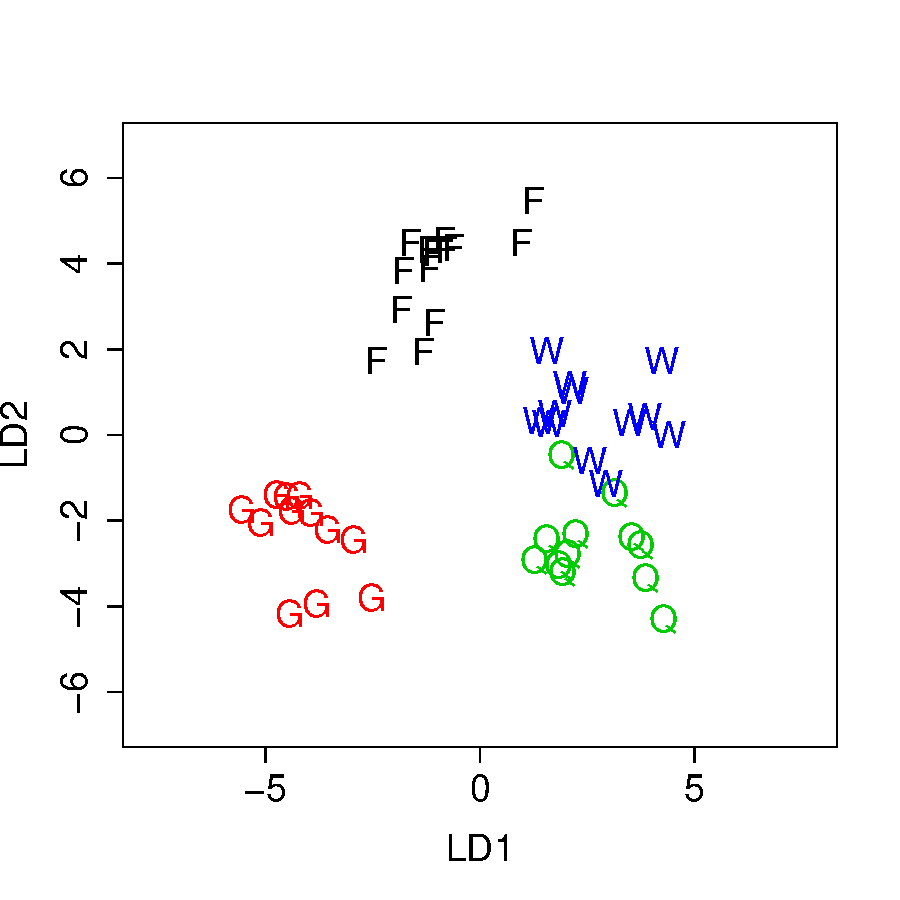
\includegraphics{toth_lda.pdf}}
       \caption{LD1 versus LD2 from an LDA on a randomly selected subset of 40 significantly different oligos : F, Foundress; G, gyne; Q, queen and W, worker. It can be noticed that the groups F and G are separated. This plot is generated to match Figure 2 in \cite{toth:2010}. }
     \label{oligo}
%\end{figurehere}
\end{figure*}  

%Any statistical analysis must include some statistical graphics. For exploratory data analysis, statistical graphics play an invaluable role in model checking and diagnostics. Even though we have established mathematical procedures to obtain various statistics, we need to support the results by also producing the relevant plots. \\
%topic
%{\color{red} Recent advancements in statistical graphics. How statistical graphics has been recently used as a tool for statistical inference.}\\
%In recent times there have been major advances in statistical graphics. Modern computing systems like R and SAS produce high quality statistical graphics. 


%{\color{red} Explanation of Large p, Small n}\\
%A challenging case of data mining is the high dimensional, low sample size (HDLSS) data. In HDLSS  settings, the number of dimensions of the data is larger or often much larger than the number of observations. HDLSS data occur in many applied areas like microarray analysis, face recognition and gene expression data. As pointed out in \cite{marron:2007}, classical multivariate statistical methods often fail to give a meaningful analysis in HDLSS contexts. 


%Let us consider the following example of LDA method used to classify the groups of paper wasps. There are 50 different paper wasps divided into 4 groups: Foundress (F), Gyne (G), Queen (Q) and Worker (W). There are 14 paper wasps of type Foundress and 12 each of the other 3 types. The authors, knowing that LDA requires that the number of observations ($n$) should be larger than ($p$), randomly selected a subset of 40 significantly different oligonucleotides from a total of 447 oligonucleotides. Figure \ref{oligo} shows the scatterplot of LD1 versus LD2.

%\newpage

%Figure \ref{oligo} clearly shows that groups Foundress(F) and Gyne(G) are two separated clusters while the groups Worker(W) and Queen(Q) are not separated and forms a separate cluster. It would be interesting to find whether the separation is real or fake.

%topic
%{\color{red} Outline of the paper.}

This paper describes visual statistical inference as applied to dimension reduction for HDLSS. In particular we focus on dimension reduction using projection pursuit, and the effect that having large dimension has on the robustness of the separation between groups.  Small simulation experiments are used to examine the problem in a controlled setting. The next section explains visual inference methods. Section \ref{sec:dimred} discusses the dimension reduction methods. Section \ref{sec:experiment} discusses the experiment designed to examine people's perception of separation in the presence of real separation and ``purely noise" for simulated HDLSS data and also provides the theoretical explanation behind the choice of dimensions for the experiment. Amazon's Mechanical Turk (\cite{turk}) was used to conduct the experiment. Section \ref{sec:results} analyze the collected data and provide results. The wasps data is revisited at the end of the paper. 
%In this paper we check the projection pursuit optimization on pure noise with no real separation by using statistical graphics in Section \ref{sec:largep}. We also check the PP optimization on dimensions with some real separation and present results. In Section  \ref{sec:distance} we are also concerned about how the distance between the means increase with $p$ for a fixed n. We also present a probable range for the number of dimensions at which the clusters starts to separate out for both one dimensional and two dimensional projections.


%\section{Visual Statistical Inference} \label{sec:visual_test} 
%
%This section outlines the concepts of visual inference in comparison to the procedures of classical statistical inference. 
%
%Let $\theta$ be a population parameter of interest, with $\theta \in \Theta$, the parameter space. 
%Any null hypothesis $H_0$ then partitions the parameter space into $\Theta_0$ and $\Theta_0^c$, with $H_0: \theta \in \Theta_0$ versus $H_1: \theta \in \Theta_0^c$. 
%% In hypothesis testing terminology, the parameter space $\Theta$ of a population parameter $\theta$, can be partitioned into $\Theta_0$ and $\Theta_0^c$. We test $H_0: \theta \in \Theta_0$ versus $H_1: \theta \in \Theta_0^c$.
%
%%\subsection{Visual Statistic} 
%
%Unlike classical hypothesis testing, the statistic in visual inference is not a single value, but a plot that is appropriately chosen to describe the parameter of interest, $\theta$. When the alternative hypothesis is true, it is expected that the plot of the observed data, the test statistic, will have visible feature(s) consistent with $\theta \in \Theta_0^c$, and that visual artifacts will not distinguish the test statistic as different when $H_1$ is not true.
%
%\begin{dfn}\label{dfn:lplot}
%A lineup plot is a layout of $m$ visual statistics, consisting of 
%\begin{itemize}\itemsep-3pt
%\item $m-1$ plots simulated from the model specified by $H_0$  (null plots) and 
%\item the test statistic produced by plotting the observed data, possibly arising from $H_1$.
%\end{itemize}
%\end{dfn}
%
%If $H_1$ is true, the test statistic is expected to be the plot that is most different from the other plots in the lineup plot. A careful visual inspection should reveal the differences in the feature shown by the test statistic under null and alternative hypothesis. {\em If the test statistic cannot be identified} in the lineup, the conclusion is to {\em not reject the null hypothesis.} The $(m-1)$ null plots can be considered to be samples drawn from the sampling distribution of the test statistic assuming that the null hypothesis is true.
%
%
%Since the lineup plot consists of $m$ plots, the probability of choosing any one of them is $1/m$. Thus we have type-I error probability of $1/m$.
%
%The lineup plot can be evaluated by one or more individuals. When a single individual identifies the observed graph in the lineup plot we report a $p$-value smaller than $1/m$, otherwise the $p$-value is larger than $1/m$. 
%
%If $N$ individuals evaluate a lineup plot independently, we count the number of successful evaluations as $U \sim \text{Binom} (N,\frac{1}{m})$ and report a  $p$-value of at most $Pr(U \ge u)= \sum_{k \ge u}^N {{N \choose k} (\frac{1}{m})^k(1-\frac 1m)^{(N-k)}}$ where $u$ is the observed number of successful evaluations. %Notice that when $N=1$, this $p$-value is $\frac1m$. 
%
%
%For two different visual test statistics of the same observed data, the one  is better, in which a specific pattern is more easily distinguishable visually.

%\section{Inference for the means of two populations} \label{sec:largep}
\section{Visual inference methods} \label{sec:inference}

\cite{buja:2009} proposed two protocols, namely rorschach and lineup,  that allow the testing of discoveries made from statistical graphics. While the Rorschach protocol helps understand the extent of randomness, the lineup protocol is particularly used for testing significance of findings. This method is called visual statistical inference. \cite{majumder:2011} made a head to head comparison between visual statistical inference tests versus classical tests which yielded comparable results. Unlike classical hypothesis testing, the test statistic in visual inference is not numeric, but a plot that is appropriately chosen which displays a very distinctive pattern in case that the null hypothesis is not true. The lineup protocol embeds the observed data plot amongst the null plots. Null plots are created by a method consistent with the null hypothesis. Human subjects are asked to identify the plot which has the most distinct feature(s). If the human subjects can identify the plot of the observed data, null hypothesis is rejected. When the alternative hypothesis is true, it is expected that the plot of the observed data, the test statistic, will have visible feature(s) inconsistent with the null hypothesis and human subjects will be able to identify the plot of the observed data as different from all the other null plots. 

As for example, suppose we have this data that represents the concentration of a metal in mg/kg for two sites A and B.
%Model : $Y_i$ = $\beta_0$ + $\beta_1 X_i$ + $\epsilon_i$, \qquad $\epsilon_i \stackrel{iid}{\sim} N(0, \sigma^2)$ \\
%\vspace{0.1cm}
We want to test whether there exists a significant difference between the concentration levels in the two sites A and B. Let $\mu_1$ denote the mean concentration level in Site A and $\mu_2$ denote the mean concentration level in Site B. Thus the null and alternative hypothesis would be
\[
H_o: \mu_1 = \mu_2 \qquad \hbox{versus} \qquad H_a: \mu_1 \ne \mu_2
\]
%\vspace{0.4cm}
We choose the visual test statistic to be a dot plot of the observed data for two groups as shown in Table \ref{tbl:compare}. The null plots are generated by assuming that $H_o$ is true. This is achieved by randomly permuting the values of group variable site and keeping the other variables fixed. The observed data plot is placed randomly among 19 null plots to obtain a lineup shown in Figure \ref{lineup}. If $H_0$ is not true, there should be a vertical displacement of the plot which would be a distinctive feature that should not be present in the null plots. The lineup is shown to the human observer and asked to identify the plot that is most different than others in the lineup. If the observer can identify the plot of the real data, there will be reasons to believe that the observed data plot has a pattern which is absent in the null plots. So the null hypothesis would be rejected. If the viewer cannot identify the observed data plot, we fail to reject the null hypothesis. A comparison of visual test with conventional test is shown in Table \ref{tbl:compare}.
%\newpage

\begin{figure}[hbtp]
%\begin{figurehere}
   \centering
       \scalebox{1}{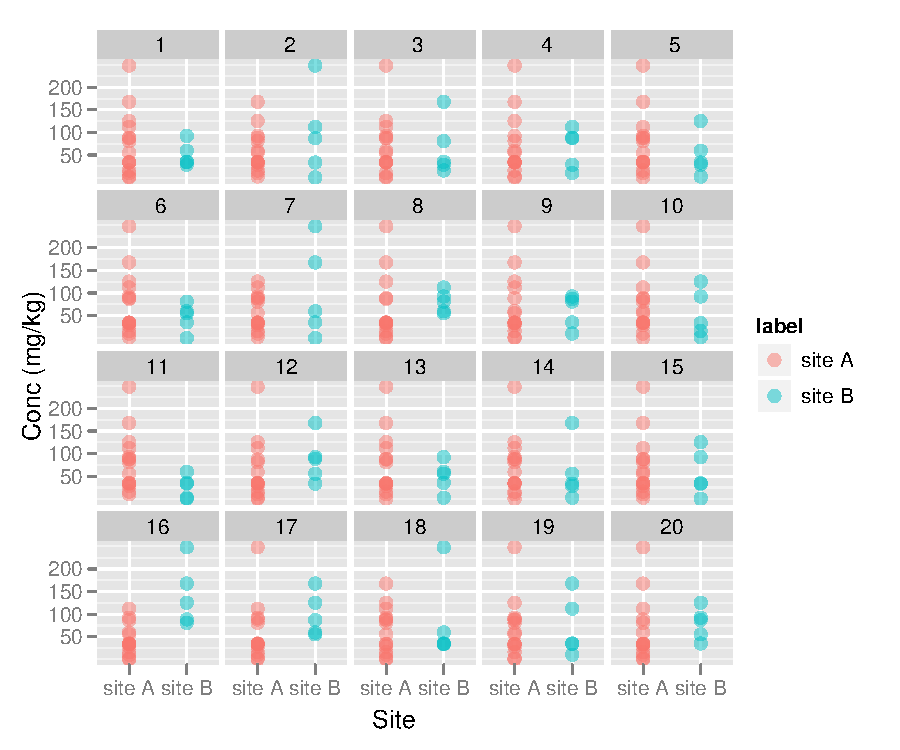
\includegraphics{lineup-dot.pdf}}
      \caption{A typical lineup  ($m = 20$) for testing $H_o: \mu_1 =  \mu_2$. 
      % \qquad vs \qquad H_a: \beta_1 \ne 0$
      When the alternative hypothesis is true the observed data plot should have the largest vertical difference between the centers. Can you identify the observed data plot? The solution to the lineup is provided in the Appendix.}
      \label{lineup}
%	\vspace{-.1in}
\end{figure}

%\newpage

%If the viewer could identify the plot then there are reasons to believe that there exists a statistically significant difference between the mean concentration levels in site A and site B. So the lineup protocol is the basis of the visual inference while the Rorschach protocol helps viewer understand the extent of randomness. 

\cite{majumder:2011} describes the methods of obtaining the power of the visual test. For their simulation experiments they recruited human observers from Amazon Mechanical Turk \citep{turk} and estimated power from human evaluations of lineups. They also obtained the power theoretically with an assumption supported by the experimental data. The result suggests that the power of visual statistical inference is comparable to conventional tests in a setting of testing the parameters of linear regression models. The subject specific power of the visual test is also estimated from the multiple responses data from each human observer. 

%\cite{majumder:2011} describes a comparative study between the visual inference method and the classical inference methods, focusing on plots that might be used in linear modeling. In his work the expected power of the visual test is compared with the power of the uniformly most powerful (UMP) test. The power of the visual test is computed by responses from several large samples of lineup evaluators recruited through Amazon Turk \citep{turk}. The results suggest that the expected power of a visual test is almost as good as the power of UMP test, that visual inference compares favorably with classical testing, in the traditional setting where the classical test performs well. They established properties and efficacy of visual testing procedures in order to use them in situations where traditional test cannot be used. In addition \cite{majumder:2011} provide a nice way of making the leap from traditional hypothesis testing to visual inference. The table is adapted for the $H_o: \mu_1 =  \mu_2$ vs $H_a: \mu_1 \ne \mu_2$ example described and plotted in Figure \ref{lineup}, which can be seen in Table \ref{tbl:compare}.

%\newpage

\begin{table*}[hbtp]
\caption{Comparison of visual inference with traditional hypothesis testing.}
\centering 
\begin{tabular}{llll} 
\hline
  & Mathematical Inference &  Visual Inference \\ %[0.5ex] % inserts table %heading 
\hline
  Hypothesis & $H_o: \mu_1= \mu_2$ vs $H_a: \mu_1 \ne \mu_2$& $H_o: \mu_1 = \mu_2$ vs $H_a: \mu_1 \ne \mu_2$\\
%  \vspace{0.5cm}	
 & \begin{minipage}[h]{1.5cm} \begin{center} \scalebox{0.25}{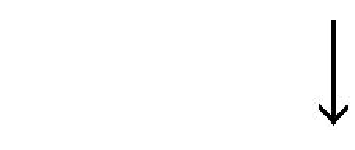
\includegraphics{down_arrow.pdf}} \end{center} \end{minipage} & \begin{minipage}[h]{1.5cm} \begin{center} \scalebox{0.25}{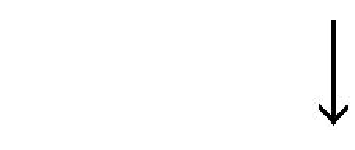
\includegraphics{down_arrow.pdf}} \end{center} \end{minipage} \\
%\vspace{0.5cm}				  
 Test Statistic & $T(y)=\frac{\bar{y}_1 - \bar{y}_2}{s\sqrt{\frac{1}{n_1} + \frac{1}{n_2}}}$ & $T(y)=$ \begin{minipage}[h]{1cm} \begin{center} \scalebox{0.35}{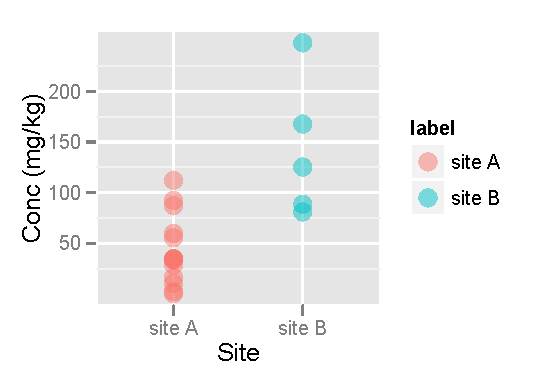
\includegraphics{data-dot.pdf}} \end{center} \end{minipage} \\
				 
 & \begin{minipage}[h]{1.5cm} \begin{center} \scalebox{0.25}{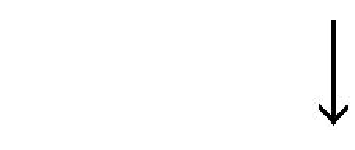
\includegraphics{down_arrow.pdf}} \end{center} \end{minipage} & \begin{minipage}[h]{1.5cm} \begin{center} \scalebox{0.25}{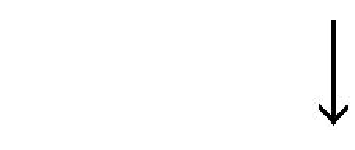
\includegraphics{down_arrow.pdf}} \end{center} \end{minipage} \\
				 
 Sampling Distribution & $f_{T(y)}(t); $\begin{minipage}[h]{1.5cm} \begin{center} \scalebox{0.5}{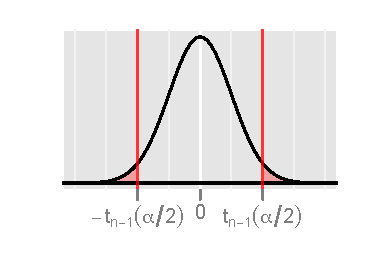
\includegraphics{two-sided-rejection.pdf}} \end{center} \end{minipage} & $f_{T(y)}(t); $ \begin{minipage}[h]{1.5cm} \begin{center} \scalebox{0.29}{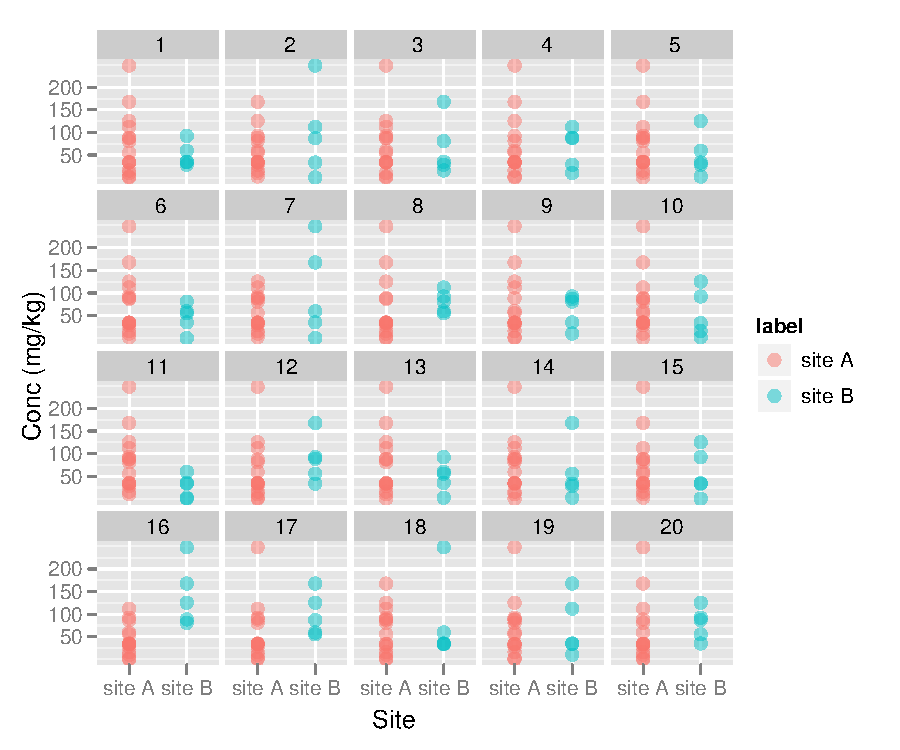
\includegraphics{lineup-dot.pdf}} \end{center} \end{minipage} \\
 & \begin{minipage}[h]{1.5cm} \begin{center} \scalebox{0.25}{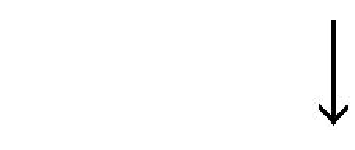
\includegraphics{down_arrow.pdf}} \end{center} \end{minipage} & \begin{minipage}[h]{1.5cm} \begin{center} \scalebox{0.25}{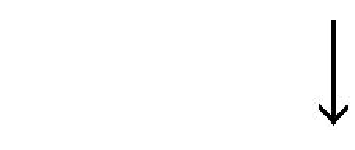
\includegraphics{down_arrow.pdf}} \end{center} \end{minipage} \\
 Reject $H_o$ if & observed $T$ is extreme & observed data plot is identifiable \\
\hline 
\end{tabular}
\label{tbl:compare}
\end{table*}

%Visual Inference can be used to test a number of hypothesis for which a classical test is unknown till date. Later in 2012, \cite{majumder:2011} does a comparative study of the empirical power of the classical test and the visual test and shows that visual test does a reasonable job in a classical situation. But in situations where the classical test is unknown till date, the visual test still maintains a good power. 


%, and that visual artifacts will not distinguish the test statistic as different when the alternative hypothesis is not true.

%{\blue *** Fill this section in. Doesn't need too much, needs to have basics and refer to Buja and  Mahbub's paper, and your tech reports.}

%\section{Theoretical expectation of dimension reduction for HDLSS data} \label{sec:theory}

%\subsection{Motivation}

%\section{Explanation of the methods}

 
\section{Explanation of dimension reduction methods}  \label{sec:dimred}

%$$\bar{\bf{X}}_{i.}^*$$

%{\color{red} Explanation of Projection Pursuit(Dimension Reduction)} \\
In this work projection pursuit (e.g. \cite{friedman:1974}) is used for dimension reduction. Projection pursuit (PP) finds the most interesting low dimensional projection from high dimensional data by maximizing some criterion of interest, e.g. variance or clustering or group separation. In this paper the one and two dimensional projections are obtained by projection pursuit.  As pointed out in \cite{huber:1985} the most exciting feature of projection pursuit is that it can bypass the curse of dimensionality. 

In classification problems, linear discriminant analysis (LDA) can be used to find a low-dimensional space where the groups are most separated. This corresponds to using the LDA index (\cite{lee:2009}) in projection pursuit:

Let $\bf{X_{ij}}$ be the $p$-dimensional vector of the $j$th observation in the $i$th class, $i = 1, \dots, g, j = 1, \dots, n_i$, $g$ is the number of classes, $n_i$ is the number of observations in class $i$, and $n = \sum_{i = 1}^g n_i$. Let $\bar{\bf{X}}_{i.} = \frac{1}{n_i} \sum_{j = 1}^{n_i} \bf{X}_{ij}$ be the $i$th class mean and $\bar{\bf{X}}_{..} = \frac{1}{n} \sum_{i = 1}^g \sum_{j = 1}^{n_i} \bf{X}_{ij}$ be the total mean. Let

$$\hbox{\bf{B}} = \sum_{i=1}^g n_i (\bar{\bf{X}}_{i.} - \bar{\bf{X}}_{..})(\bar{\bf{X}}_{i.} - \bar{\bf{X}}_{..})^T : \hbox{between-class sum of squares}$$

$$\hbox{\textbf{W}} = \sum_{i=1}^g \sum_{j=1}^{n_i} (\bf{X_{ij}} - \bar{\bf{X}}_{i.})(\bf{X_{ij}} - \bar{\bf{X}}_{i.})^T : \hbox{within-class sum of squares}$$
Then, the LDA PP index is 

$$
I_{LDA}(\hbox{\bf{A}}) = \left\{ \begin{array}{cc}
 1 - \frac{\left|\hbox{\textbf{A}}^T \hbox{\bf{W}} \hbox{\bf{B}}\right|}{\left|\hbox{\bf{A}}^T \left(\hbox{\textbf{ W }} + \hbox{\textbf{ B }}\right)\hbox{\textbf{A}}\right|} &\mbox{ for $|\bf{A}^T(\bf{W} + \bf{B})\bf{A}| \neq 0$} \\
 0 &\mbox{ for $|\bf{A}^T(\bf{W} + \bf{B})\bf{A}| = 0$}
       \end{array} \right.
$$
where \textbf{A} is an orthogonal projection onto a $k$-dimensional space.

For HDLSS data, the penalized discriminant analysis (PDA) index (\cite{lee:2009}) is more robust:

Let ${\bf{X}}_{ij}^*$ be the standardized vector of ${\bf{X}}_{ij}$. Then 

$$
\hbox{\bf{B}}^s = \sum_{i=1}^g n_i (\bar{\bf{X}}_{i.}^* - \bar{\bf{X}}_{..}^*)(\bar{\bf{X}}_{i.}^* - \bar{\bf{X}}_{..}^*)^T : \hbox{between-class sums of squares of the standardized data}
$$

$$\hbox{\bf{W}}^s = \sum_{i=1}^g \sum_{j=1}^{n_i} ({\bf{X}}_{ij}^* - \bar{{\bf{X}}}_{i.}^*)({{\bf{X}}_{ij}^*} - \bar{\bf{X}}_{i.}^*)^T : \hbox{within-class sums of squares of the standardized data }$$
where $\bar{{\bf{X}}}_{i.}^*$ is the $i$th class mean of the standardized data and $\bar{\bf{X}}_{..}^*$ is the total mean of the standardized data. Then the PDA index is defined as

$$I_{PDA}(\hbox{\bf{A}},  \lambda) = 1 - \frac{|\hbox{\bf{A}}^T\{(1 - \lambda))\hbox{\bf{W}}^s + n\lambda I_p\}\hbox{\bf{A}}|}{|\hbox{\bf{A}}^T\{(1 - \lambda))(\hbox{\bf{W}}^s + \hbox{\bf{B}}^s) + n\lambda I_p\}\hbox{\bf{A}}|}$$
where \textbf{A} is an orthonormal projection onto a $k$-dimensional space and $\lambda \in [0, 1)$ is a predetermined parameter. Penalized LDA (\cite{witten:2011}) is another approach.

These indices are available for projection pursuit using the \texttt{tourr} package in \texttt{R} (\cite{r}) (\cite{WC08}). The \texttt{tourr} package produces tours of multivariate data. The package also includes functions for creating different types of tours like grand, guided and little tours, which project multivariate data with $p$ dimensions to 1, 2, 3 or $d$ dimensions where $d \le p$. The guided tour function is used here. The guided tour will converge to a maximally interesting projection, here that is one where groups show the biggest separation.     

%{\color{red} Statement of the problem. What we want to show. }\\

%The optimization procedure in the  \texttt{tourr} package is new, different from the algorithms that have existed before in GGobi \cite{STLBC03} and XGobi \cite{SCB91}. 
%We have been using PP with the PDA index, on a large $p$, small $n$ data set from a microarray study, and for comparison have been looking at pure noise data. As strange as it might seem it seemed like we could often pick the projection of the  ``original'' data from a lineup of projections of permuted class data. This should not be possible.
%
%The distance between clusters obtained by doing a LDA or a PDA on a noise data increases as we increase the number of dimensions $p$ for a fixed sample size $n$. So another motivation for this paper is in situations where the number of dimensions ($p$) is approximately equal or close to the number of observations ($n$), we may see separation among the groups when a linear discriminant analysis (LDA) or a penalized discriminant analysis (PDA) is performed. A natural question is whether there is actually a real separation among the groups or we observed the separation due to the fact that $p \approx n$ or $p > n$. 
%
%To check the optimization procedure we looked at the absolute difference of the means of random noise divided into two groups. We start with one dimensional data of random noise and assign two groups. Since we are interested in the projections, we work with the absolute differences of the means. \\

%\newpage


%%%%%%%%%%%%%

%In this paper, data with $p$ dimensions of noise and no real separation is termed as ``$p$ dimensional purely noise data'' while data which has $k$ dimensions of real separation and $p - k$ dimensions of purely noise is termed as ``$p$ dimensional data with k dimension(s) of real separation''. In this paper $k$ is either 1 or 2. 


\section{Experiment} \label{sec:experiment}

\subsection{Experimental design}

%{\blue*** Explain the Turk experiment}

The goal of the experiment was to determine how well real separation is distinguishable from random noise. To achieve this goal, the experiment was set up with factors, real separation or purely noise, dimension and projection dimension. Real separation was achieved by setting 1 or 2 variables with real separation among a number of purely noise variables.  Sample size was fixed to keep the experiment manageable. Also mean shift was kept fixed. The levels of the factors used in the experiment are given in Table \ref{freq}. Three replicates at each level were generated. These produced 60 different ``observed data sets", and thus, 60 different lineups. 

\begin{table}[htbp]
\begin{center}
\caption{Levels of the factors used for the experiment.}
\begin{tabular}{cccp{2.2cm}|c}
  \hline
  \hline
  $n$ & projection($d$) & separation & dimension ($p$) & replicates\\
  \hline
  30 & 1 & Yes & 20, 40, 60, 80, 100 & 3 \\
      & & No & 20, 40, 60, 80, 100 & 3\\
   30 & 2 & Yes & 20, 40, 60, 80, 100 & 3 \\
     & & No & 20, 40, 60, 80, 100 & 3\\   
      \hline
\end{tabular}
\label{freq}
\end{center}
\end{table} 

Figure \ref{fig:dimen} shows the distribution of absolute difference of means for data with separation and without separation for different dimensions. The distributions of data with and without separation are shown in blue and red respectively. The area of the distribution of purely noise which is above the 5th percentile of the distribution of data with separation is shown in dark blue and the dark blue region increases with dimension ($p$). This indicates that as dimension increases, the distributions of data with or without separation gets closer. Hence the probability of obtaining separation among groups for purely noise data increases with higher dimensions. Fixing the area of the dark blue region and calculating the dimensions to obtain the required region provides the choice of levels of dimension. More details are provided in Section \ref{sec:theory}. 

\begin{figure}[hbtp]
%\begin{figurehere}
   \centering
       \scalebox{0.70}{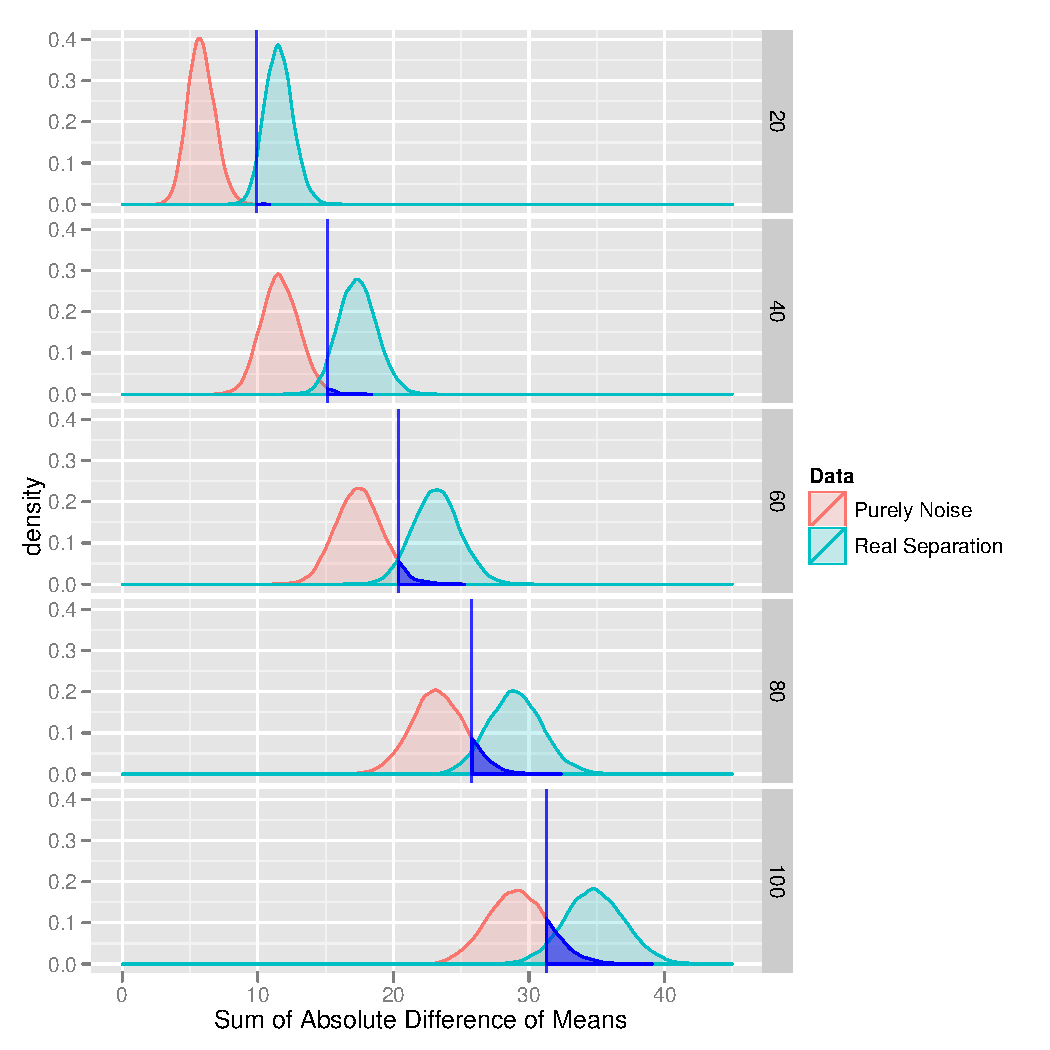
\includegraphics{sum-noise-real-2.pdf}}
       \caption{Plot showing the distribution of the sum of absolute difference of means for data with and without separation for different dimensions. The distributions of data with real separation ($Z$) and purely noise data ($Y$) are shown in blue and red respectively with the dark blue line showing the 5th percentile of $Z$. The dark blue area shows the area of $Y$ which is greater than the 5th percentile of $Z$. The dark blue region increases as dimension ($p$) increases indicating that the probability of obtaining the sum of absolute difference for data with purely noise similar to that for data with real separation increases with $p$. }
     \label{fig:dimen}
%\end{figurehere}
\end{figure}

\subsection{Simulation process}

Two groups of $p$ dimensions of data with 15 observations in each group are generated from $N(0, 1)$.  The data from the first group is labeled as group 1 and the data from the second group as group 2. So a $30 \times (p + 1)$ matrix, say, $\mathbf{X}$, is obtained where the first 15 observations are from group 1 and the last 15 observations are from group 2. The data for both the groups is purely noise, having no dependence on the groups. So $\mathbf{X}$ can be written as
$$\mathbf{X}^{n \times (p + 1)} = (\mathbf{X}_1, \mathbf{X}_2, \dots, \mathbf{X}_p, \hbox{Group})$$ where each $\mathbf{X}_i$ is a vector of dimension 30 for $i = 1, \dots, p$. This matrix $\mathbf{X}$ excluding the Group variable gives the $p$-dimensional purely noise data or data with no separation with 2 groups.

To introduce real separation in the data, values for $p$-th variable $\mathbf{X}_p$ were shifted apart by 6 units between the two groups. So, 
$$
\mathbf{X}_p = \left\{ \begin{array}{rl}
 \mathbf{X}_p - 3 &\mbox{ if $ \mathbf{X}_p \in$ group 1} \\
 \mathbf{X}_p + 3 &\mbox{ if $ \mathbf{X}_p \in$ group 2}
       \end{array} \right.
$$

Hence two sets of data are obtained, each with $p$ dimensions with $n = 30$ observations in each dimension divided into two groups. One of the datasets is purely noise and the other has some real separation in the form of the $p$-th dimension, i.e. data with separation. On each of these datasets of $p$ dimension, a projection pursuit optimization with a PDA index is performed to obtain the $d = 1$ dimensional projection of best separation, yielding $\mathbf{Y = XA}$.  

The above procedure is effectively the same for $d = 2$ dimensional projections with few key differences. The first 10 observations is assigned as group 1, the second 10 observations as group 2 and the last 10 as group 3.  So, collectively,  $\mathbf{X}$ can be written as
$$ \mathbf{X}^{n \times (p + 1)} = ( \mathbf{X}_1,  \mathbf{X}_2, \dots, \mathbf{X}_p, \hbox{Group})$$ where each $ \mathbf{X}_i$ is a vector of dimension 30 for $i = 1, \dots, p$. This matrix $X$ excluding the Group variable gives the $p$-dimensional noise data or data with no separation with 3 groups.

To introduce real separation, the means of the 3 groups are adjusted in the last two dimensions i.e. $ \mathbf{X}_{p-1}$ and $ \mathbf{X}_p$. The adjustment is done in the following way:
$$
( \mathbf{X}_{p-1},  \mathbf{X}_p) = \left\{ \begin{array}{rl}
 ( \mathbf{X}_{p-1} - 3,  \mathbf{X}_p) &\mbox{ if $( \mathbf{X}_{p-1},  \mathbf{X}_p) \in$ group 1} \\
 ( \mathbf{X}_{p-1} + 3,  \mathbf{X}_p) &\mbox{ if $( \mathbf{X}_{p-1},  \mathbf{X}_p) \in$ group 2} \\
 ( \mathbf{X}_{p-1} ,  \mathbf{X}_p + \sqrt{27}) &\mbox{ if $( \mathbf{X}_{p-1},  \mathbf{X}_p) \in$ group 3}
       \end{array} \right.
$$
If $ \mathbf{X}_{p-1}$ versus $ \mathbf{X}_p$ are plotted in a scatterplot, the points cluster along the vertices of an equilateral triangle of side 6. Excluding the group variable, $ \mathbf{X}$ works as the data with real separation in the last two dimensions. Hence the data with 2 dimensions of real separation divided into 3 groups is obtained.  So for obtaining the two dimensional projections two sets of data are obtained - one with purely noise and the other with two dimensions of real separation. On each of the above datasets, a projection pursuit with a PDA index is performed to obtain the $d = 2$ dimensional projection of best separation, yielding $\mathbf{Y = XA}$. 

\subsection{Producing lineups}

Two different visual test statistics, $T_1(\bf{Y})$ and $T_2(\bf{Y})$ (as defined in \cite{majumder:2011}) are used in this paper, for representing 1D and 2D data. $T_1(\bf{Y})$ is a horizontal jittered dot plot, with color representing groups. $T_2(\bf{Y})$ is a scatterplot of the two-dimensional projections, with color representing groups. The same symbol is used to represent the groups in both the test statistics so that the different symbols do not confound our analysis. Figure \ref{fig3} shows the two different visual test statistics.

\begin{figure}[htbp]
\centering
\mbox{\subfigure[$T_1(\bf{Y})$]{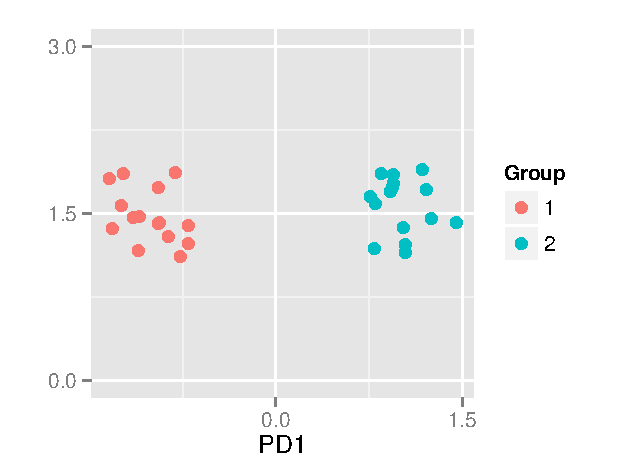
\includegraphics[width=2.5in]{test_statistic_1.pdf}}\quad
\subfigure[$T_2(\bf{Y})$]{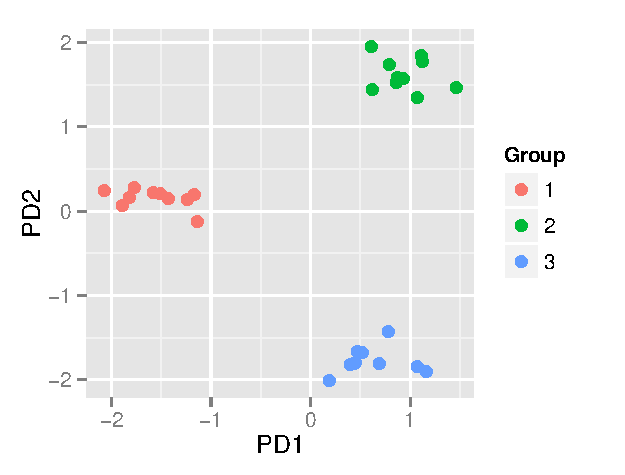
\includegraphics[width=2.5in]{test_statistic_2.pdf} }}
\caption{The visual test statistics $T_1(\bf{Y})$ and $T_2(\bf{Y})$ used in this paper.  $T_1(\bf{Y})$ is a horizontal jittered dot plot while $T_2(\bf{Y})$ is a scatterplot of the first and second dimensional projections, with color representing groups in both cases. } 
\label{fig3}
\end{figure}

%\begin{figure}[htbp]
%\centering
%\begin{subfigure}[b]{0.5\textwidth}
%\centering
%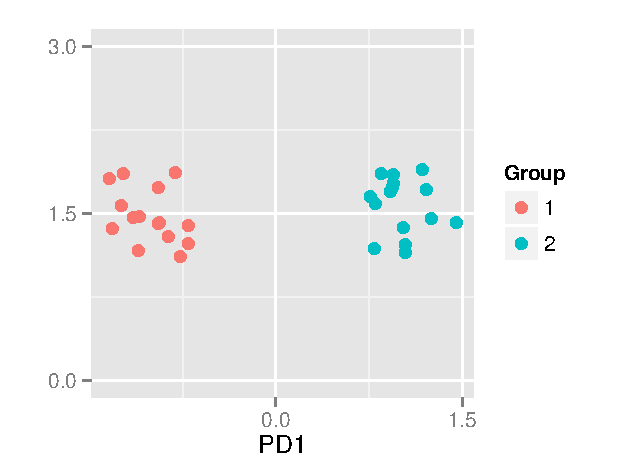
\includegraphics[0.45]{test_statistic_1.pdf}
%\caption{}
%\label{teststat1}
%\end{subfigure}
%
%\begin{subfigure}[b]{0.5\textwidth}
%\centering
%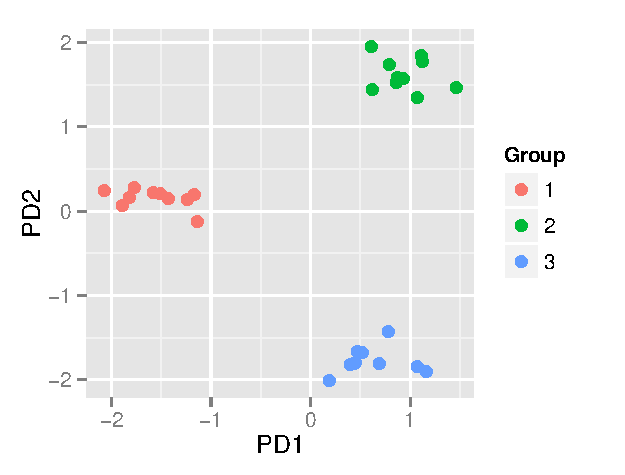
\includegraphics[0.45]{test_statistic_2.pdf}
%\caption{}
%\label{teststat2}
%\end{subfigure}
%
%\label{teststat}\caption{This is the figure}
%
%
%\end{figure}

To obtain the 19 null plots in a lineup of size $m = 20$, the group variable is permuted in order to break any dependence between the group variable and the other variables and the projections are obtained and plotted in the same way, as the test statistic. The test statistic, which is the observed data plot, is placed randomly among the 19 null plots. To maintain the same orientation of the two groups in the 1D projection lineup,  the mean of the projections for each group is calculated for each plot in the lineup and the group with the lower mean is considered as group 1 and the other as group 2. Figure \ref{fig:test_category_1d} shows an example lineup  from treatment with $p = 20$, separation = Yes and $d = 1$. Similarly, Figure \ref{fig:test_category} shows an example lineup for $p =100$, separation = No and $d = 2$.

A statistic WBratio which is the ratio of the average distance within clusters to the average distance between clusters (\cite{hennig:2010}) is calculated for each plot in the lineup of both 1D and 2D projections. An additional statistic Wilk's $\lambda$ (\cite{JW02}) is calculated for 2D projections. Projection pursuit is an optimization routine and there are occasional problems of convergence with two-dimensional projections. To account for this problem, 30 null plots are generated. The 19 null plots which have the smallest Wilk's $\lambda$ values are used for the lineup. 

%{\color{red} The data recorded for the participants. How many participants were recruited.} \\

% and Figure \ref{not_noise_1d} gives the lineup plot for the one dimensional projections for 99 dimensions of pure noise and 1 dimension of real separation.
% and Figure \ref{not_noise} gives the lineup plot for the two dimensional projections for 98 dimensions of pure noise and 2 dimensions of real separation.

%\end{multicols}
%
\begin{figure}[hbtp]
%\begin{figurehere}
   \centering
       \scalebox{1.00}{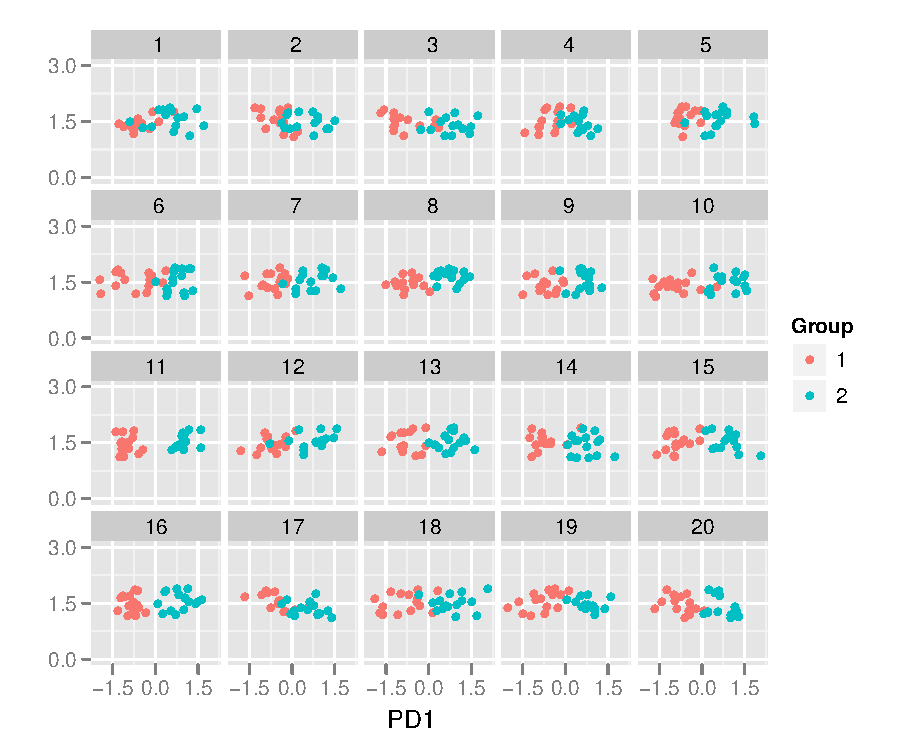
\includegraphics{plot_real_1d_20_11.pdf}}
       \caption{Lineup  ($m=20$) from treatment with $p = 20$, separation = Yes and $d = 1$. The subjects were asked to identify the plot with the most separated colors. Can you identify the observed data plot? The solution to the lineup is provided in the Appendix. }
     \label{fig:test_category_1d}
\end{figure}


 
\begin{figure}[hbtp]
%   \centering
       \scalebox{1.00}{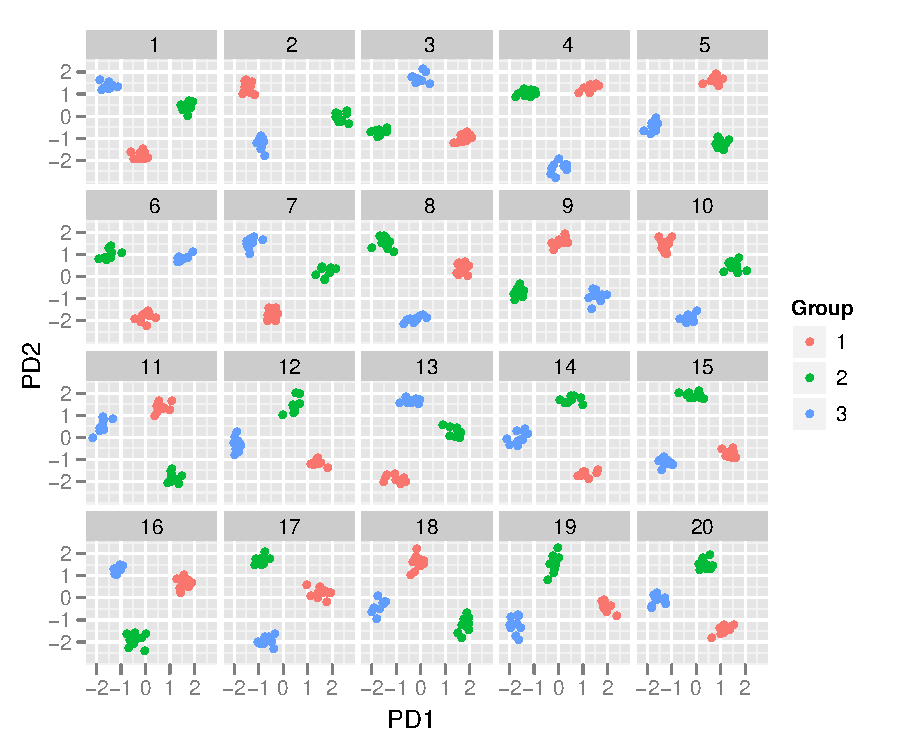
\includegraphics{plot_2d_100_15.pdf}}
       \caption{Lineup  ($m=20$) from treatment with $p = 100$, separation = No and $d = 2$.The subjects were asked to identify the plot with the most separation between the colored groups. Can you identify the observed data plot? The solution is provided in the Appendix. }
       \label{fig:test_category}
\end{figure}

%\ppp

\subsection{Data collection}

Subjects  for the experiment were recruited through Amazon Mechanical Turk  \citep{turk}. Each subject was shown a sequence of 10 lineups. Subjects also had the freedom of answering more than 10 lineups. They were asked to identify the plot which has the most separation between the colored groups. Their response was recorded along with a reason for their choice of the plot and the level of confidence they have in their decision.  Gender, age, educational qualification and location of each subject were also noted. In total, 1137 lineups were evaluated by 103 subjects, from different locations across the globe.


%\begin{figure*}[hbtp]
%%\begin{figurehere}
%   \centering
%       \scalebox{1.00}{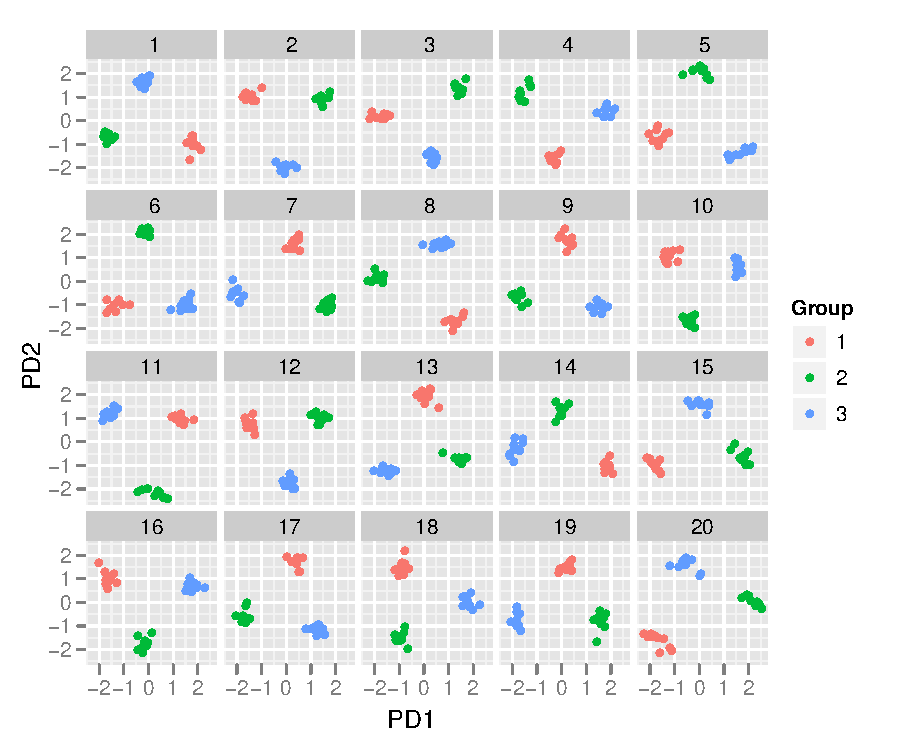
\includegraphics{plot_2d_98_5.pdf}}
%       \caption{Lineup plot ($m=20$) with 98 dimensions of pure noise and 2 dimensions of real separation for testing $H_0$: There is no difference among the plots. When the alternative hypothesis is true the observed data plot should have the largest separated colors. Can you identify the observed data plot?}
%       \label{not_noise}
%\end{figure*}


%{\color{red} Description of the procedure. }\\


%The optimization is checked for 1D and 2D projections. For 1D projections data of size 30 is simulated from a standard normal distribution with $ p=20, 40, 60, 80$ and $100$ which are close to the values obtained in Table \ref{tab:dimen}. The first 15 observations are labeled class 1 and the second 15 observations are labeled class 2. There is no true class, it is pure noise data -- any separation seen between classes in the projection are purely due to the high dimension. We compute projection pursuit using the PDA index and plot the one dimensional projections in a lineup plot with $m=20$ where alternatives plots are created by randomly permuting the class labels. We expect that the original data should not be detectable -- it's just noise, any labeling of the observations to class is random. 

%topic
%{\color{red} Statement of the problem. What we want to show. }\\
%Consider two random samples $X_{i1}, X_{i2}, \dots, X_{ip}$ for $i = 1$ and 2 which have means $\mu_1 = (\mu_{11}, \mu_{12}, \dots, \mu_{1p})^T$ and $\mu_2 = (\mu_{21}, \mu_{22}, \dots, \mu_{2p})^T$ respectively. We consider testing the following high-dimensional hypothesis :
%
%$$H_0 : \mu_1 = \mu_2 \qquad \hbox{versus} \qquad H_a : \mu_1 \neq \mu_2 .$$
%
%The hypothesis $H_0$ consists of the $p$ marginal hypotheses $H_{0l} : \mu_{1l} = \mu_{2l}$ for $l = 1, \dots, p$ regarding the means on each data dimension.
%
%%The optimization procedure in the  \texttt{tourr} package is new, different from the algorithms that have existed before in GGobi \cite{STLBC03} and XGobi \cite{SCB91}. 
%%We have been using PP with the PDA index, on a large $p$, small $n$ data set from a microarray study, and for comparison have been looking at pure noise data. As strange as it might seem it seemed like we could often pick the projection of the  ``original'' data from a lineup of projections of permuted class data. This should not be possible. 
%
%\subsection{Procedure}
%topic

%For testing the above hypothesis, we simulate two sets of $p$-dimensional data from a standard normal distribution with $n = 15$ observations in each dimension in each set. Consider $Z_{ij} = (Z_{i1}, Z_{i2}, \dots, Z_{ip})$ for $i = 1$ and 2 and $j = 1, \dots, p$ are simulated from a $N(0, 1)$ distribution. These  two sets of data should represent the random samples collected from the two population. To test for the equality of means, we bring in some separation in the last dimension by adding and subtracting a value $\delta$ from the mean of the dimensions.  
%
%We define $X_{1p} = - \delta + Z_{1p} $ and $X_{2p} = \delta + Z_{2p}$. 
%We bring in a class variable which indicates the population the dataset is obtained from. The first 15 observations are labeled class 1 and the second 15 observations are labeled class 2.  We compute projection pursuit using the PDA index and plot the one dimensional projections in a lineup plot with $m=20$ where alternatives plots are created by randomly permuting the class labels.  We showed the lineup plots to several subjects and asked them to identify the plot which has the largest separation among the groups.
%
%To compare the above method, we again simulate two sets of $p$-dimensional data from a standard normal distribution with $n = 15$ observations in each dimension in each set. So now we have $X_{ij} = Z_{ij}$ for $i = 1$ and 2 and $j = 1, \dots, p$. So the two datasets from the two population do not have any real separation and they are pure noise. We again compute using the PDA index and plot the one dimensional projections in a lineup plot with $m=20$ where alternatives plots are created by randomly permuting the class labels. Several individuals were again asked to identify the plot which has the largest separation among the groups.\\[1cm]
%
%
%{\color{blue}Do not know how to write the two dimensional projections in this set up. May be test for equality of mean vectors for 3 populations ??}


%For 2D projections data is simulated from a standard normal distribution with $ p=20, 40, 60, 80$ and $100$ with 30 observations in each dimension. The first 10 observations are labeled class 1, the second 10 observations are labeled class 2 and the last third are labeled class 3. There is no true class, it is pure noise data. To account for the occasional convergence problem with the optimization 30 null plots are generated. The 19 null plots which have the smallest Wilks $\lambda$ (\cite{JW02}) values are used for the lineup. 
%
%For comparison, for each of these examples we also simulated data that had real classes, too. We also simulated data with ($p$ - 1) dimensions of pure noise and one dimension of real separation, in all making it $p$ dimensions. In the same way, each dimension has  30 observations and they were divided into 2 classes. The separation was designed in a way such that if we plot the one dimension with real separation, the points lie approximately 6 units apart. Once again the first 15 observations are labeled class 1 and the last 15 observations are labeled class 2. In this case there is one dimension of real separation. We once again compute the projection pursuit using the PDA index and plot the one dimensional projections.
%
%For 2D projections, data is simulated $p$ dimensions of pure noise. Again each dimension has  30 observations with 3 classes. But in this case the last two dimensions are changed so that the data has some real separation. The two dimensions with real separation was constructed such that the points lie close to the vertex of an equilateral triangle of side 6 units. Once again the first 10 observations are labeled class 1, the second 10 observations are labeled class 2 and the last third are labeled class 3. Here we have two dimensions of real separation. We again compute projection pursuit using the PDA index and plot the two dimensional projections in a lineup plot.  To account for the occasional convergence problem of optimization we select the 19 plots with the minimum Wilk's $\lambda$ from the generated 30 plots generated.



%\begin{multicols}{2}

%\section{Visual Inference and HDLSS Experiment}\label{sec:experiment}
%%topic
%\subsection{Procedure}

%{\color{red} Description of the experiment. How the experiment was conducted. What are the parameters, how many different plots.} \\
%An experiment is designed to study the ability of human observers to detect the effect of one dimension of real separation in $p$ dimensions of noise. Data is simulated for different values of $p$  ( = 20, 40, 60, 80, 100) with sample size $ n  =  15$. For bringing in the real separation, we fixed $\delta $ = 3. So two sets of $p$ dimension of data with sample size $n = 15$ were generated from Normal(0 ,1) for the two populations.  $\delta = 3$ was added and subtracted to the $p$-th dimension to bring in the largest separation.  We also repeated the above procedure for the different $p$ dimensions of pure noise with no real separation ($\delta = 0$). Data sets with different combinations of $n$, $p$ and presence of noise were generated with frequencies shown in Table \ref{freq}. Three replicates of each level were generated.These produced 30 different ``observed data sets''. 
%
%%({\color{blue} only for one dimensional projections.}) 
%
%\begin{table}[htbp]
%\begin{center}
%\caption{Values of parameters considered for the experiment.}
%\begin{tabular}{cccp{3cm}}
%  \hline
%  \hline
%  $n$ & projection & presence of real separation & $p$ \\
%  \hline
%  15 & 1 & Y & 20, 40, 60, 80, 100 \\
%      & & N & 20, 40, 60, 80, 100\\
%   10 & 2 & Y & 20, 40, 60, 80, 100 \\
%     & & N & 20, 40, 60, 80, 100\\   
%      \hline
%\end{tabular}
%\label{freq}
%\end{center}
%\end{table}
%topic
%{\color{red} How the null plots were generated. }\\
%The 19 null plots in the lineup were obtained by  permuting the population indicator variable (the variable that indicates which population the data set belongs to) so that breaking any dependency between the indicator variable and the other variables. Two different statistics Wilk's $\lambda$ (\cite{JW02})  and the within sum of squares to between sum of squares ratio were calculated for each of the 20 plots in the lineup. \\
%{\color{red} The data recorded for the participants. How many participants were recruited.} \\
%Participants  for the experiment were recruited through Amazon Mechanical Turk. Each participant was shown a sequence of 9 lineups. They were asked to identify the plot which has the most separation between the colored groups, give a reason for their choice and determine the level of confidence for their decision.  Gender, age, educational qualification and location of each participant were also noted. In total, 1137 lineups were evaluated by 103 participants from different locations. \\



\section{Results} \label{sec:results}

%topic
%{\color{red} Description of the results. }\\

%Participants  for the experiment were recruited through Amazon Mechanical Turk ( \cite{turk} ).  \cite{turk} is an amazing platform to get feedback on this kind of experiments. Each participant was shown a sequence of 10 lineups. Participants also had the freedom of answering more than 10 lineups. They were asked to identify the plot which has the most separation between the colored groups. Their response was recorded along with a reason for their choice of the plot and the level of confidence they have in their decision.  Gender, age, educational qualification and location of each participant were also noted. In total, 1137 lineups were evaluated by 103 participants from different locations.

\subsection{Data cleaning}

Amazon Mechanical Turk subjects were paid for their responses. Since the process was not manually monitored, some subjects did not make an honest effort to find the observed data plot. To counter this problem, each subject was given a very easy lineup (a lineup with $p = 10$ dimensions with some real separation). The subjects who failed to give a correct response to this lineup were removed from the study. If their response in this lineup was correct, we remove the subject's response for this lineup but keep all their responses for all the other 9 lineups viewed.

\subsection{Effect of experimental factors} \label{effects}

We would expect that subjects are correct more often when there is real separation and that as dimension increases, correctness decreases. Figure \ref{suc-rate-glm} examines this. The proportion correct is plotted against the different levels of dimension faceted by the levels of separation and projection. The 3 different dots for each level shows the 3 replicates for each level combination of the factors. The line represents the fitted fixed effects logistic regression model. The success rate is higher for low dimensions, and decreases as dimension increases, for real separation for both 1D and 2D projections. For noise data, the success rate is flat across dimensions. There also appears to be increasing variance as dimension increases.

%It can be noticed that when there is some real separation, the rate of success in making the correct response overall is higher. Also there is a difference in terms of the variability among the replicates in each dimension.
% The rate of success is not very different for 1D and 2D projections both in case of data with real separation and also for noise data. %\subsection{1D vs 2D projections}
%Also with the different values of the dimension $p$, the rate of success in picking the correct plot is different. The rate is higher for dimension $p = 20$ than when the dimension is $p = 40$. Strangely enough it can be noticed that the rate of success for $p = 100$ is higher than the rate of success for $p=80$ for both 1D and 2D projections. 

\begin{figure}[ht]
%\begin{figurehere}
   \centering
       \scalebox{0.6}{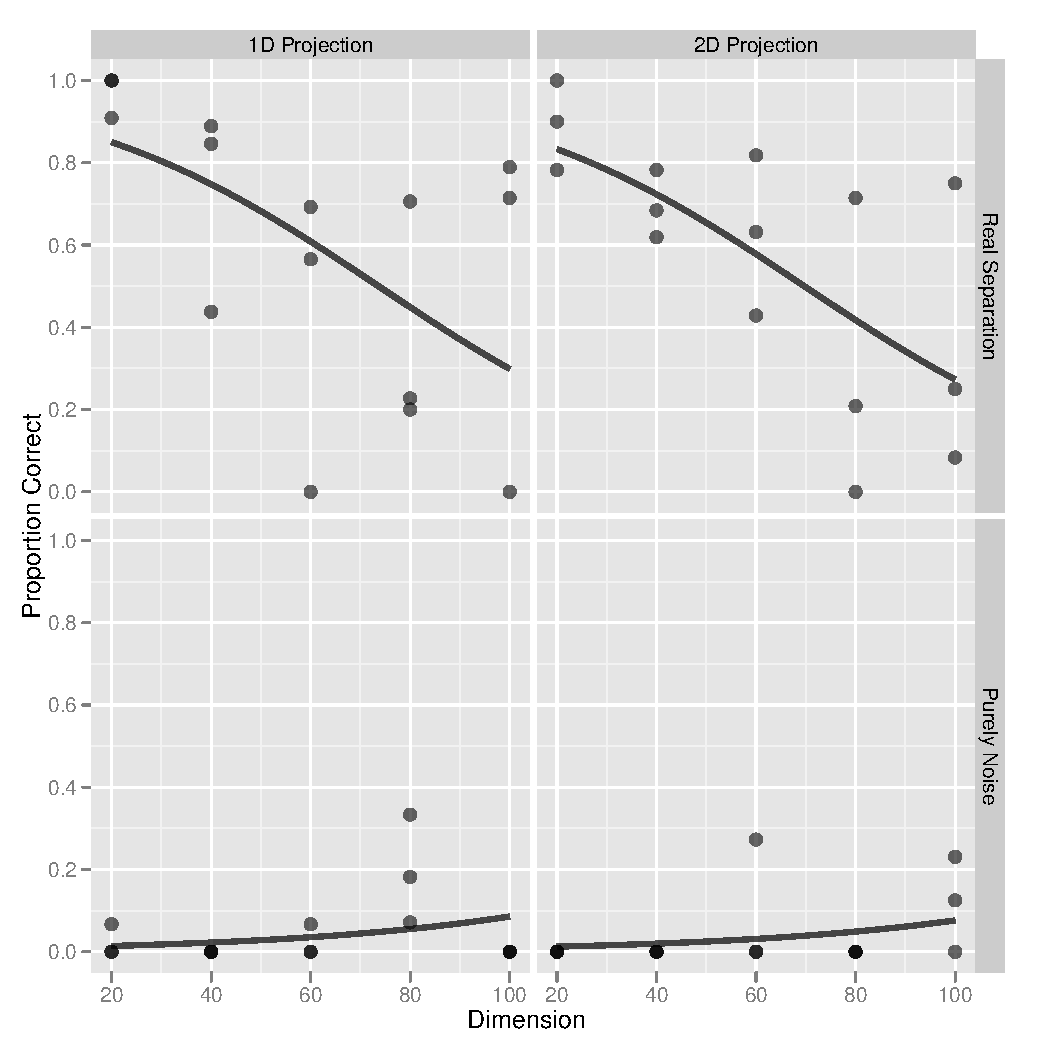
\includegraphics{suc-rate-rep-int-glm.pdf}}
%        \scalebox{0.80}{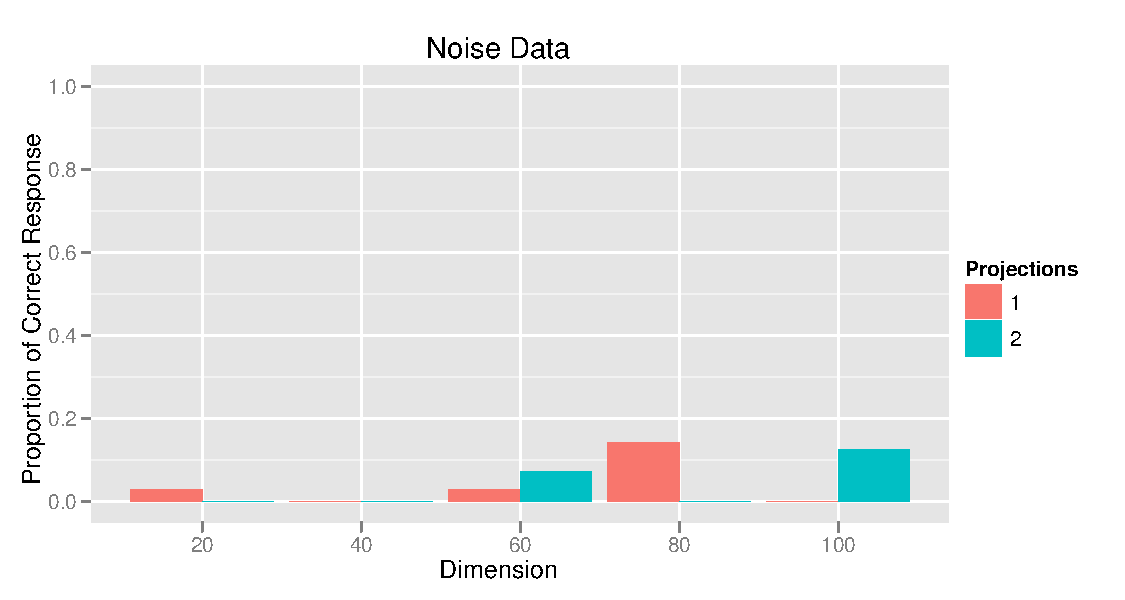
\includegraphics{result-noise.pdf}}
      \caption{Proportion of correct response against dimension faceted by projection and separation. The three points represents the three replicates for each treatment level. A fixed effects logistic regression model is overlaid on the points. It can be seen that the success rate decreases as dimension increases for data with real separation. When the data is purely noise data, the success rate is flat across dimensions. The success rate does not change with projection.  }
       \label{suc-rate-glm}
\end{figure}

%\subsection{Model fitting}

%Suppose each of $K$ independent subjects responded to multiple lineups and responses are considered to be a binary random variable $Y_{lk}$ where $$Y_{lk} \sim \hbox{Ber}(p_{lk})$$ where $Y_{lk} = 1$ if the $k$-th subject correctly identifies the observed data plot in the $l$-th lineup, $1 \leq k \leq K$, $1 \leq l \leq L$ and 0 otherwise. The main interest is to predict the proportion of successes by dimension. Treating dimensions as a continuous variable, a fixed effects logistic regression model is used for $P(Y_{lk} = 1) = p_{lk} = E(Y_{lk})$ with the different parameters of the lineup as covariate.
%The model can be fit as:
%\begin{equation}
%g(p_{lk}) = \theta + \alpha_{lk} + \beta_{lk} + \gamma x_{lk} + \alpha_{lk} \gamma x_{lk} \label{fixed}
%\end{equation}
%where $\theta$ is the intercept, $\alpha_{lk}$ is the effect of noise on the $l$-th lineup for the $k$-th subject,
%$\beta_{lk}$ is the effect of projection on the $l$-th lineup for the $k$-th subject 
%and $x_{lk}$ is the dimension of the $l$-th lineup for the $k$-th subject. An interaction between the effect of noise and dimension is also included in the model. $\gamma$ is the corresponding slope parameter and $g(.)$ denotes the logit link function $g(\pi)$ = log($\pi$) - log(1 - $\pi$); $0 \leq \pi \leq 1$. The logit link function is inverted to estimate the lineup specific probability of successful evaluation as 
%\begin{equation}
%\hat{p}_{lk} = g^{-1}(\hat{\theta} + \hat{\alpha}_{lk} + \hat{\beta}_{lk} + \hat{\alpha}_{lk} \hat{\gamma} x_{lk}) \label{invert}
%\end{equation}

%Model \ref{fixed}
A fixed effects logistic regression model is fitted to the data and the estimated proportions of successful evaluation for each lineup is obtained. Table \ref{params} shows the estimates of the model parameters, the standard errors and the corresponding $p$-values. We observe that the $p$-values corresponding to dimension and presence of real separation is very highly significant. The interaction term is also significant. But the $p$-value corresponding to the projection is high, which suggests that projection is not significant at 5\% level of significance. The slope of the covariate dimension is different when there is separation or not. When the observed data plot has real separation, the ability to detect it decreases with dimension, but the opposite occurs when the observed data plot has no real separation.

\begin{table}[ht]
\begin{center}
\caption{Table showing the estimate, the standard error and the $p$-value of the parameters used in logistic regression model. The covariates dimension and separation are highly significant while projection is not significant at 5\% level of significance. The interaction term between dimension and separation is also significant.}
\vspace{0.15cm}
\begin{tabular}{r|rrr}
\hline
  \hline
 Parameters & Estimate & Std. Error  & $p$-value \\ 
  \hline
Intercept  & 2.381 & 0.278  & 0.000 \\ 
  dimension($p$) & $-$0.032 & 0.004  & 0.000 \\ 
  separation = No & $-$7.097 & 0.911  & 0.000 \\ 
  projection = 2D & $-$0.127 & 0.181  & 0.483 \\ 
  separation:dimension & 0.056 & 0.011 & 0.000\\
   \hline
\end{tabular}
\label{params}
\end{center}
\end{table}


%The estimated models for the different treatment levels are provided. 
%
%$$
%g(\hat{p}_{lk}) = \left\{ \begin{array}{rl}
% 2.381 - 0.032 x_{lk} &\mbox{for data with real separation and 1D projections} \\
% -4.716 + 0.024 x_{lk} &\mbox{for data with purely noise and 1D projections} \\
%  2.254 - 0.032 x_{lk} & \mbox{for data with real separation and 2D projections} \\
%  -4.843 + 0.024 x_{lk} &\mbox{for data with purely noise and 2D projections} \\
%       \end{array} \right.
%$$
 

%\subsection{Response as the dimension increases}


%\subsection{Subject-wise responses}
%
%To look at the subject specific probability of successful evaluation Model \ref{fixed} is modified to bring in  a random effect for the individuals. Using the setup of Model \ref{fixed}, we have
%\begin{equation}
%g(p_{lk}) = \theta + \alpha_{lk} + \beta_{lk} + \gamma x_{lk} + \alpha_{lk} \gamma x_{lk} + u_k \label{mixed} 
%\end{equation}
%where $u_k$ is a random effect specific to individual $k$, $k = 1 \leq k \leq K$ and $u_k \sim N(0, \sigma_u^2)$ independently. As before the link function is inverted to obtain the probability of successful evaluations.
%
%Using \textit{lme4} package in R, a mixed effects logistic regression model is fitted as specified in Model \ref{mixed}. The thin black lines in Figure \ref{subject-glm} shows the estimated probability of successful evaluation of each individual with the blue line showing the fixed effect. It can be noticed that some of the subjects has a very high probability of success for both one and two dimensional projections. Also as the number of dimensions increases, the probability of successful evaluation decreases. Most of the individuals perform similarly when the data has no real separation. Also there is a higher variability in the individual responses for data with real separation but not much when the data is purely noise.
%
%\begin{figure*}[ht]
%%\begin{figurehere}
%   \centering
%       \scalebox{0.6}{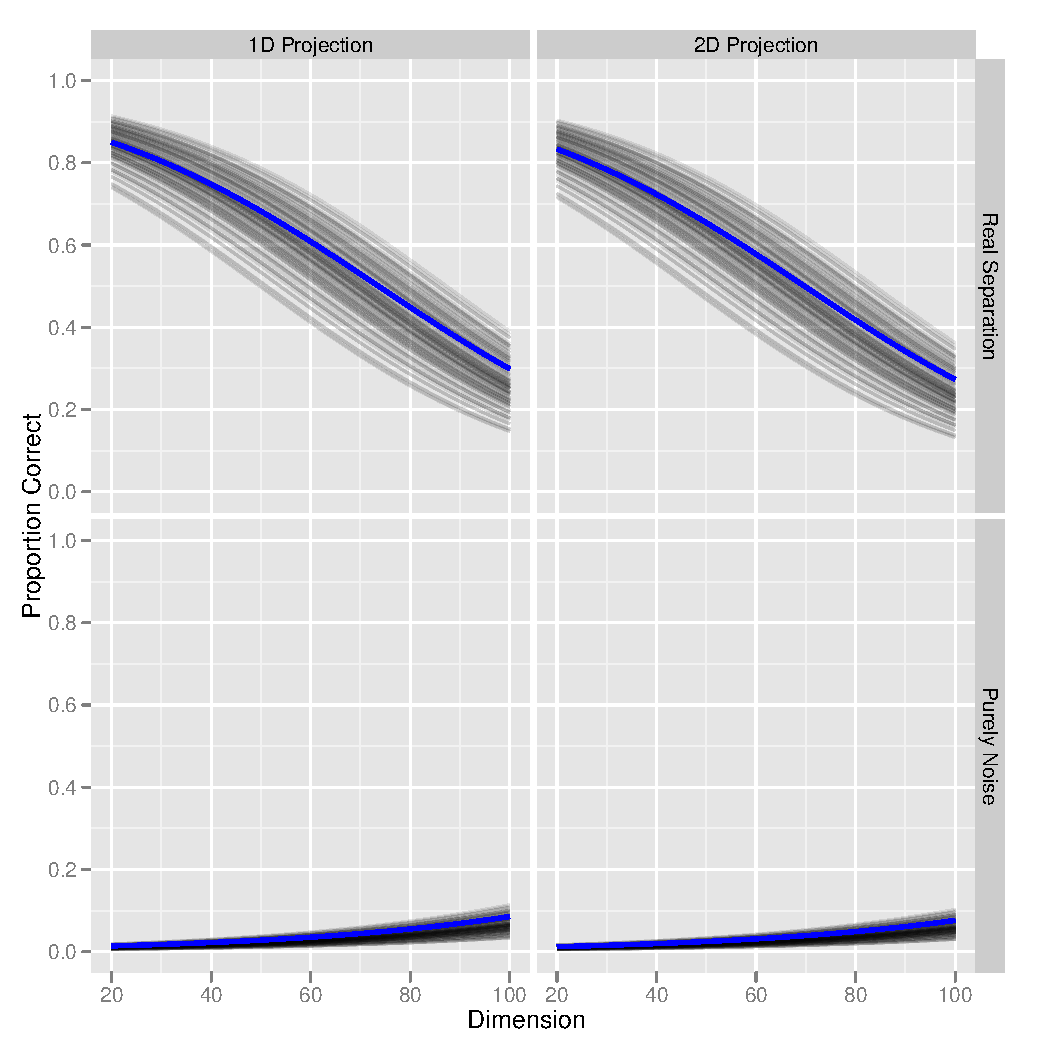
\includegraphics{subjectwise-glm-int.pdf}}
%%        \scalebox{0.80}{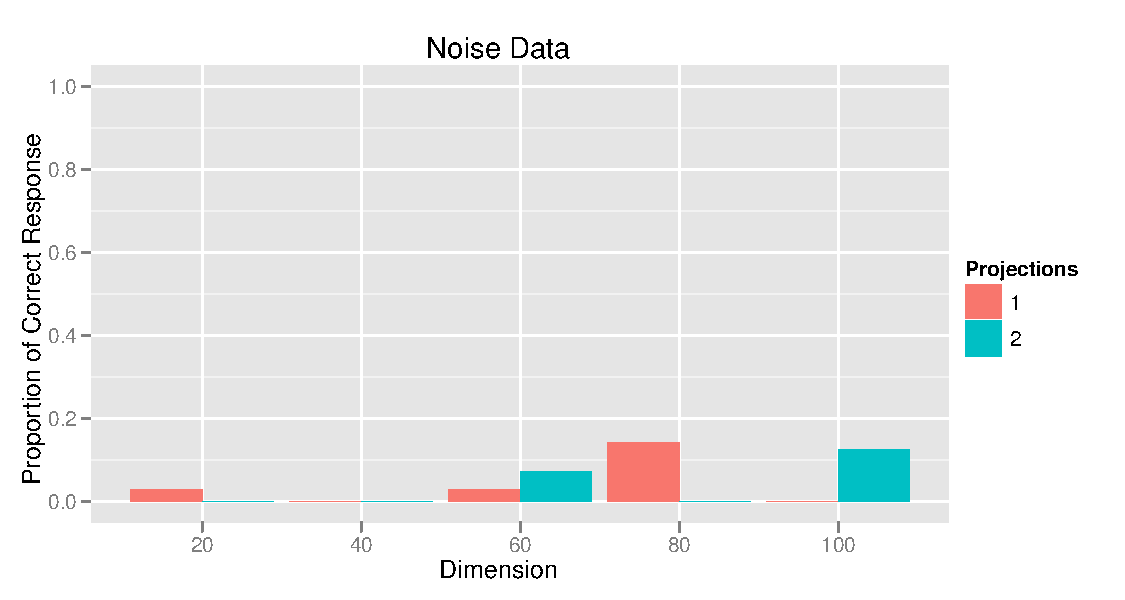
\includegraphics{result-noise.pdf}}
%      \caption{Plot showing subject wise proportions for each subject estimated using Model \ref{mixed}. The thick blue line shows the overall average proportion for all the subjects. It can be noticed that some of subjects have higher proportion of correct response than the others. }
%       \label{subject-glm}
%\end{figure*}
%
%%\newpage

\subsection{Does rotation in the 2D projections affect the responses?}

The 1D projections were plotted in a lineup making the adjustment that the group with the lower values of projection are always considered to be group 1. So the orientation of the groups does not affect the response of the subjects. But in case of 2D projections, the groups are rotated in a different way in each plot in the lineup (Figure \ref{fig:test_category}) which may influence the response of the subjects. We can check if the rotation in the 2D projections does effect the performance. Since the 1D projections are adjusted, the lineups of the 1D projections are used as a control and the responses for the 1D and 2D projections are compared. Figure \ref{suc-rate-glm} shows that there is not much of a difference between the 1D and 2D projections both in presence and absence of real separation. This is also verified in Table \ref{params} where the effect of the projections is not significant at 5\% level.  

%\newpage

\subsection{Time taken to respond}

We would expect that the amount of time taken to respond will increase the difficulty of identifying the observed data plot in a lineup. The distribution of the time taken to respond by the subjects is considered for the different parameters. Figure \ref{time-taken} shows the distribution of the time taken to respond (on log scale) by dimension and projection. The colors indicated separation. A loess smoother is added. Notice that, as the dimension increases, subjects  takes more time to respond to the lineups when the data has some real separation. But when the data is purely noise, the increase of dimension does not have any effect on the time. This suggests that as the number of dimension of noise increases with fixed number of real separation, it becomes harder to spot the observed data plot among the null plots. On the other hand, the difficulty of spotting the observed data plot for a data with purely noise does not vary with dimension. It can also be seen that the time taken when the data is purely noise is overall higher than the time taken when the data has some real separation. There is not much of a difference between the time taken for 1D and 2D projections.



\begin{figure*}[hbtp]
%\begin{figurehere}
   \centering
       \scalebox{0.6}{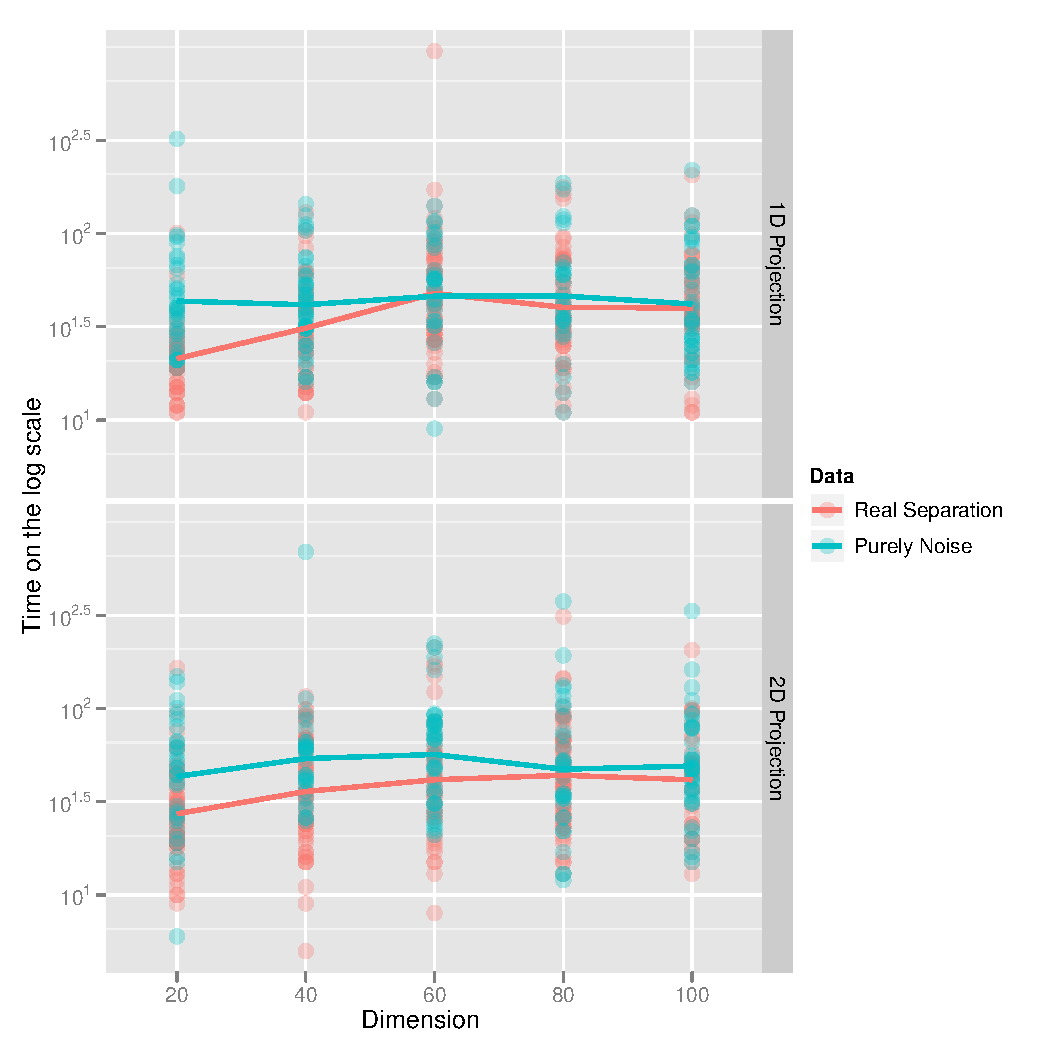
\includegraphics{time-taken-log-dot.pdf}}
%        \scalebox{0.80}{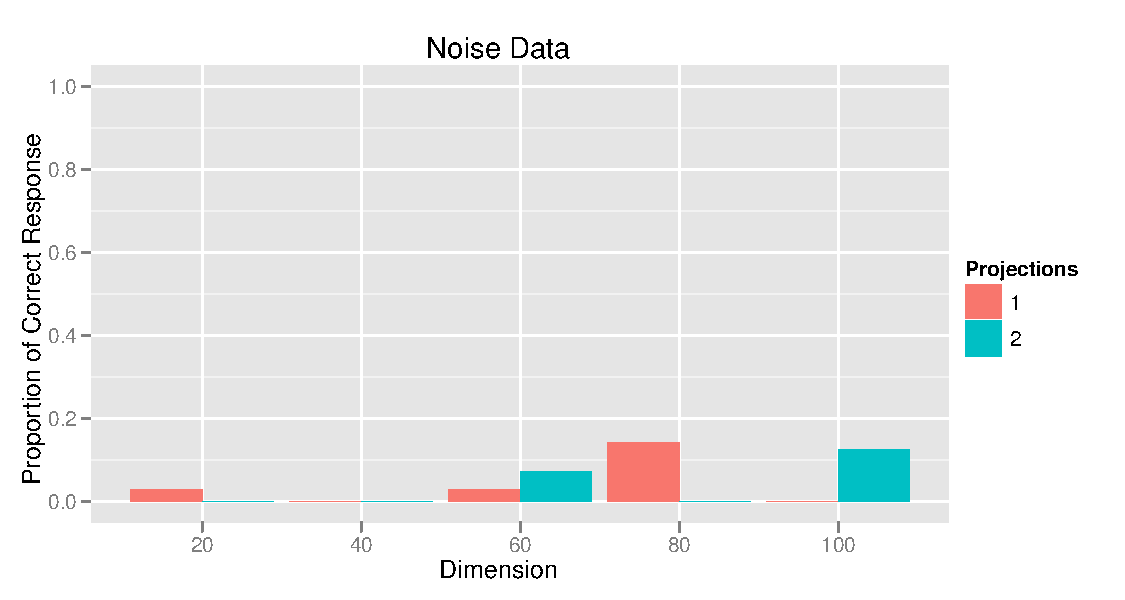
\includegraphics{result-noise.pdf}}
      \caption{Time taken to respond on log scale against dimension colored by separation and faceted by projection. A loess curve is fitted through the points for each separation and projection. Time taken to respond is higher when the data has no separation. Also as dimension increases, the difference between the time to respond for data with and without separation decreases. Subjects take more time for 2D projections.  }
       \label{time-taken}
\end{figure*}

%\begin{figure*}[hbtp]
%%\begin{figurehere}
%   \centering
%       \scalebox{0.7}{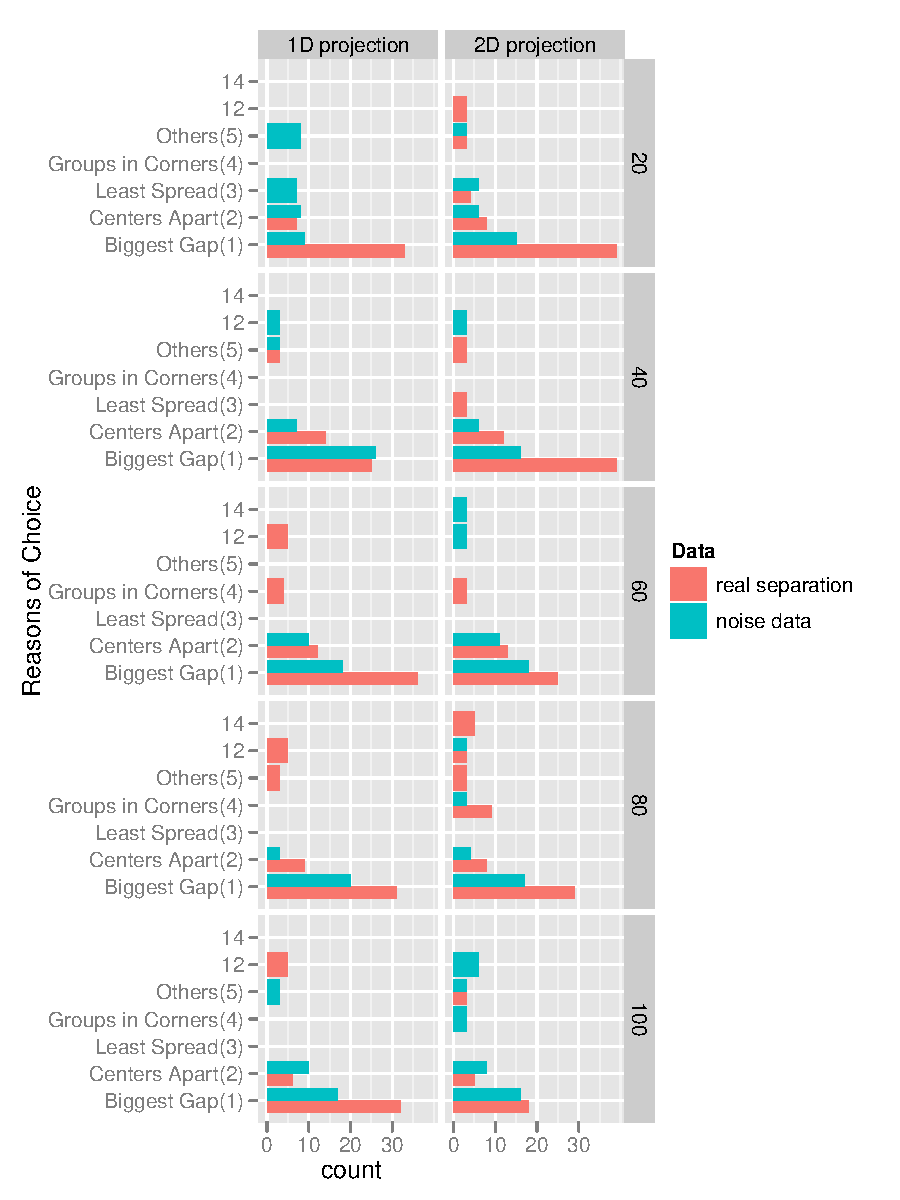
\includegraphics{choice-reason-bar.pdf}}
%%        \scalebox{0.80}{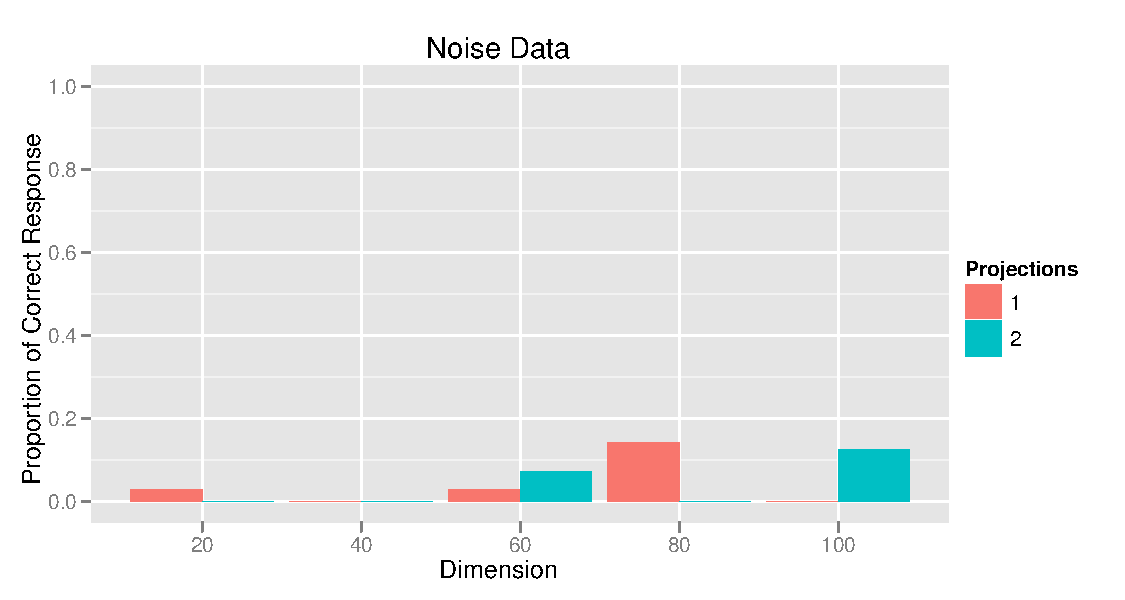
\includegraphics{result-noise.pdf}}
%      \caption{Bar diagram showing the counts of people's choice of reasons colored by the data. Notice that people mostly pick the ``biggest gap" as their choice of reason when they are working with the data with real separation. Also some of the reasons like ``Groups are in corners" does not appear for 1D projections.   }
%       \label{real_noise}
%\end{figure*}

%\Large{\textit{What affects the decision of the people?}} \\[0.2cm]

\subsection{What affects decisions?}

\normalsize
%topic
%{\color{red} What do people see when they select a plot.} \\
%Participants were asked to identify the plots which has the most separated colored groups. In data sets with real separation, participants make mistakes in picking up the plot of the ``observed data". 

Figure \ref{wbratio} examines subjects choices in depth. The relative frequency of picks of each plot in the lineup is plotted against a measure of distance separation between groups, the WBratio. %{\blue Your definition of wbratio was not correct. Check the package description, and refer to the R package, and probably the original paper describing the metric.}  
 Each cell of this figure shows data from one of the lineups used in the study, 60 in total. Each ``pin'' represents a plot in a lineup, so each cell here has 20 pins, indicating the frequency the plot was chosen. Red represents the observed data plot. Two separate figures are made for the two projections. The top three rows correspond to data containing real separation between the groups, and for the bottom three rows all of the data was purely noise. Columns indicate dimension ($p$). Replicates are in different rows. The taller the pin the more often that particular plot was chosen. We asked subjects to pick the plot where the groups were most separated, and this is effectively what they picked. The plot in each lineup with the smallest WBratio tended to have the highest frequency. This is more obvious when there was real separation, and also when dimension was small, but it is also seen in the lineups containing pure noise data. This is reassuring -- that subjects did well at detecting the biggest difference.  For some of the lineups different choices were made, and these are a little surprising. Investigating these lineups further may reveal why this is. 

%In Figure \ref{wbratio}, it can be seen that there is a negative correlation between the relative frequency of the picks and the WBratio. So as the WBratio increases, which indicates the decrease in the distance between the clusters,  the number of participants picking the plot decreases. Red dot indicates the observed data plot. For data with real separation, when the observed data plot has the smallest WBratio, the participants are successful in picking up the observed data plot. But for data with no real separation participants are able to pick the plot with the lowest WBratio value although it is not the observed data plot. Also it should be mentioned that Figure \ref{wbratio} has been drawn using a ``free scale'' along the horizontal axis. So for higher dimensions and presence of real separation and also for purely noise data, the difference between the WBratio values for different plots in a lineup are really small compared to the lineup for a lower dimension and data with real separation.  

\begin{figure}[htbp]
\centering
\mbox{\subfigure[For Projection:1D]{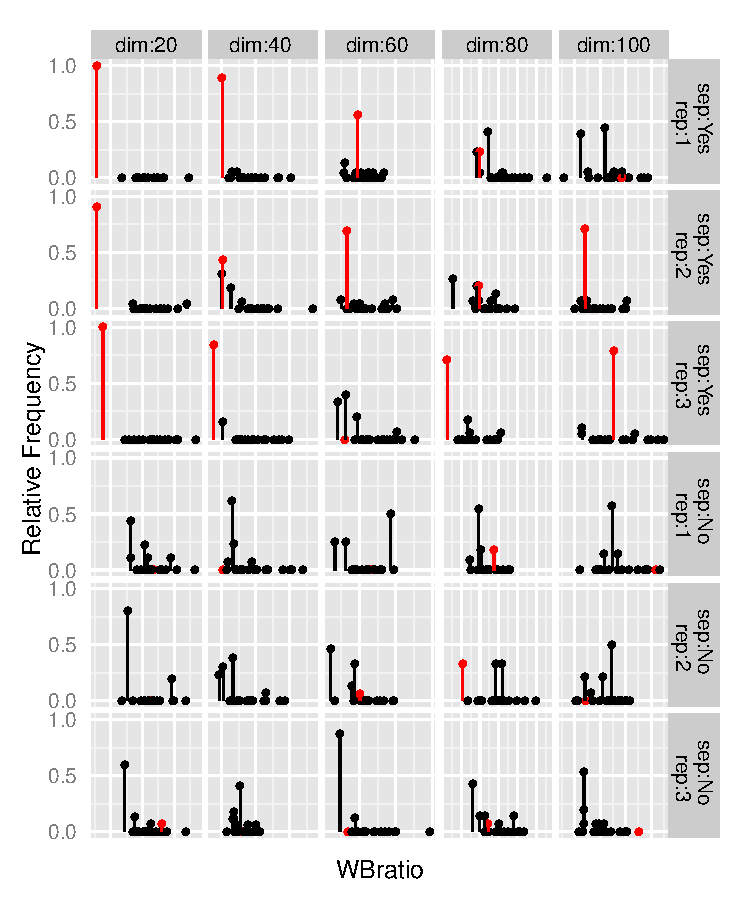
\includegraphics[width=3in]{wbratio-1.pdf}}\quad
\subfigure[For Projection:2D]{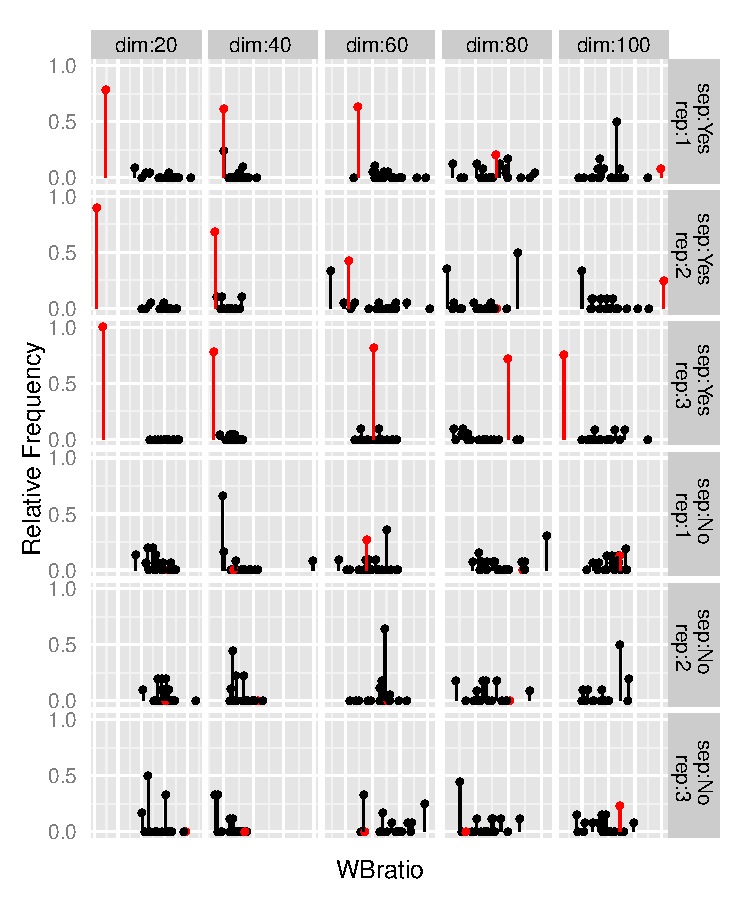
\includegraphics[width=3in]{wbratio-2.pdf} }}
\caption{Comparing the choices that subjects make for each lineup. Relative frequency of plots chosen against a measure of the distance between means, WBratio, the smaller the value the more separated are the groups. Each cell here shows the data for one of the lineups used in the experiment, 60 in total, and each ``pin'' represents a plot in the lineup, 20 for each lineup. Red indicates the observed data plot. Subjects were asked to pick the plot in the lineup where the groups were the most separated, so we would expect that more subjects would pick the plots with the smallest WBratio. In general, this happens, the tallest pins are in the left of each cell. The top three rows show the results for the data with separation, so the observed data plot (red) is typically the pin on the very left of the cell, less so for the higher dimensions which are the cells at right. Figure (a) shows 1D projections and Figure (b) shows for 2D projections. There is not much difference between the two figures. } 
\label{wbratio}
\end{figure}


%\begin{figure*}[hbtp]
%%\begin{figurehere}
%   \centering
%       \scalebox{0.63}{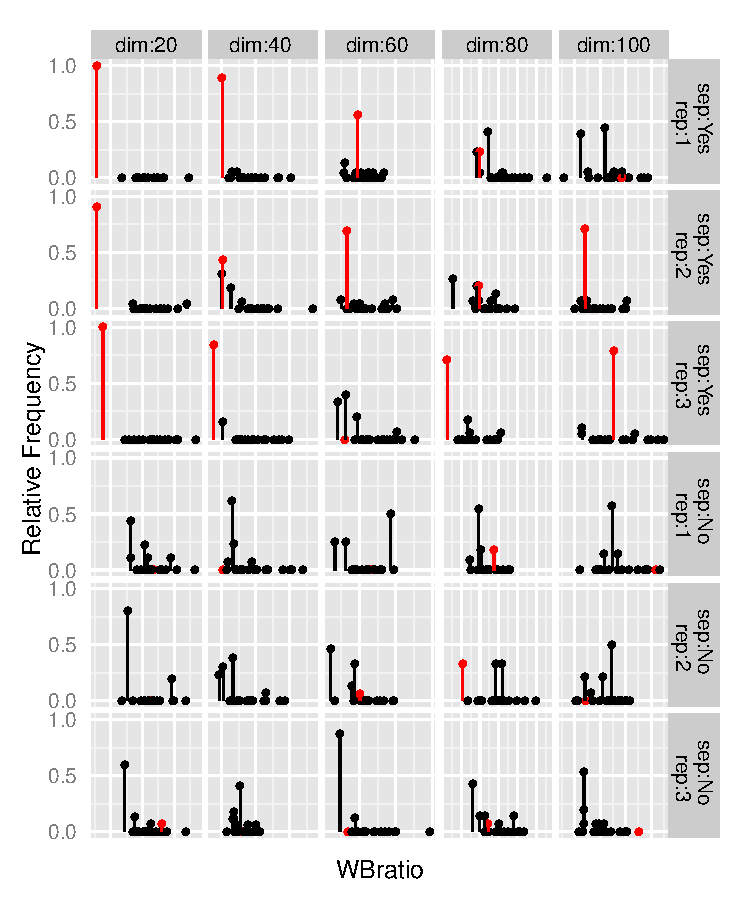
\includegraphics{wbratio-1.pdf}}
%       \scalebox{0.63}{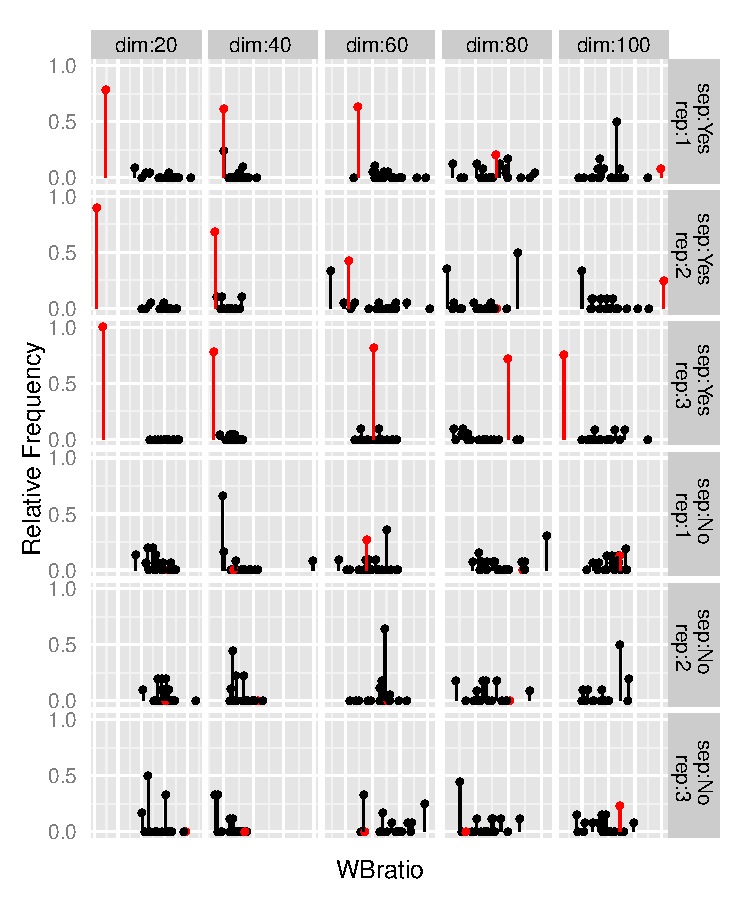
\includegraphics{wbratio-2.pdf}}
%       \caption{Comparing the choices that subjects make for each lineup. Relative frequency of plots chosen against a measure of the distance between means, WBratio, the smaller the value the more separated are the groups. Each cell here shows the data for one of the lineups used in the experiment, 60 in total, and each ``pin'' represents a plot in the lineup, 20 for each lineup. Red indicates the observed data plot. Subjects were asked to pick the plot in the lineup where the groups were the most separated, so we would expect that more subjects would pick the plots with the smallest WBratio. In general, this happens, the tallest pins are in the left of each cell. The top three rows show the results for the data with real separation, so the observed data plot (red) is typically the pin on the very left of the cell, less so for the higher dimensions which are the cells at right. Also the figure on the top is for 1D projections and on the bottom is for 2D projections. We do not see much difference between the two figures.
%       % {\blue Remove the ``of picks'' from the vertical axis. I think it would be better to have the columns grouped into 1d at the left, and 2d on the right.}
%       }
%       \label{wbratio}
%\end{figure*}

%We made 5 lineups of each of the above plots for each dimension and showed to different individuals. They were asked to pick up the ``true" one among the 20 plots. By the ``true" one, we meant the one with the most separated colors. 20\% of the individuals could identify the true plot when the data is 100 dimensions of pure noise for one dimensional projections. But when there is one dimension of separation in 100 dimensions of pure noise, 90\% of the individuals could successfully identify the true plot. For the two dimensional projections, only 30\% of the individuals could identify the true plot when the data has 100 dimensions of pure noise but 60\% of the individuals can pick the correct plot when there is two dimensions of real separation. It is evident that people are mostly correct in selecting the true plot when one dimension among 100 dimensions have real separation. People are also correct to pick the plots when two dimensions among 100 have real separation.



%\subsection{Comparisons with real separation}
%
%We also created plots with 99 dimensions of pure noise and one dimension of real separation, in all making it 100 dimensions. In the same way, each dimension has 30 observations and they were divided into 2 classes. The separation was designed in a way such that if we plot the one dimension with real separation, the points lie approximately 6 units apart. For plotting the two dimensional projections, we considered 98 dimensions of pure noise and 2 dimensions of real separation. Again each dimension has 30 observations with 3 classes. The two dimensions with real separation was constructed such that the points lies close to the vertex of an equilateral triangle of side 6 units.
%
%We made 5 lineups of such plots for each dimension and showed them to the same individuals. They were again asked to pick the plot with the most separated colors. The proportion of correct choices were 0.9 and 0.6 respectively for the one and two dimensional projections. Figure \ref{fig:result} shows the proportion of correct response by pure noise only or presence of known real separation. It is evident that people are mostly correct in selecting the true plot when one dimension among 100 dimensions have real separation. People are also correct to pick the plots when two dimensions among 100 have real separation.

%\end{multicols}

%\begin{figure}[hbtp]
%%\begin{figurehere}
%   %\centering
%       \centerline{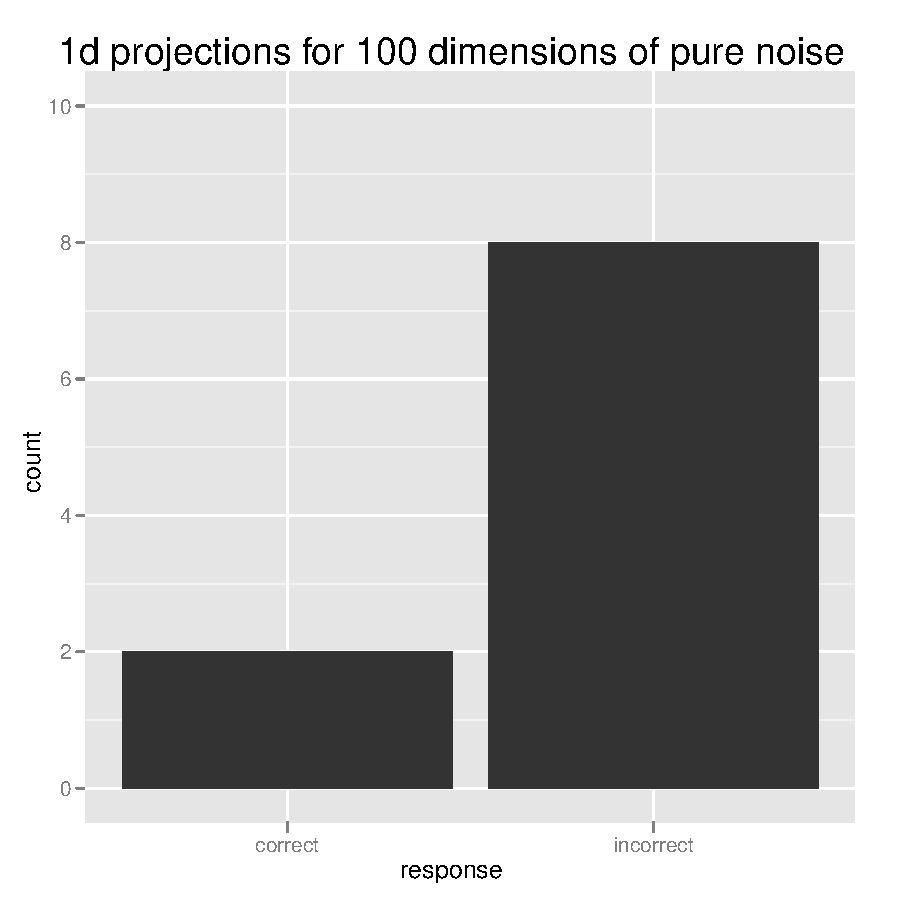
\includegraphics[width=0.25\textwidth]{result_1d_noise.pdf}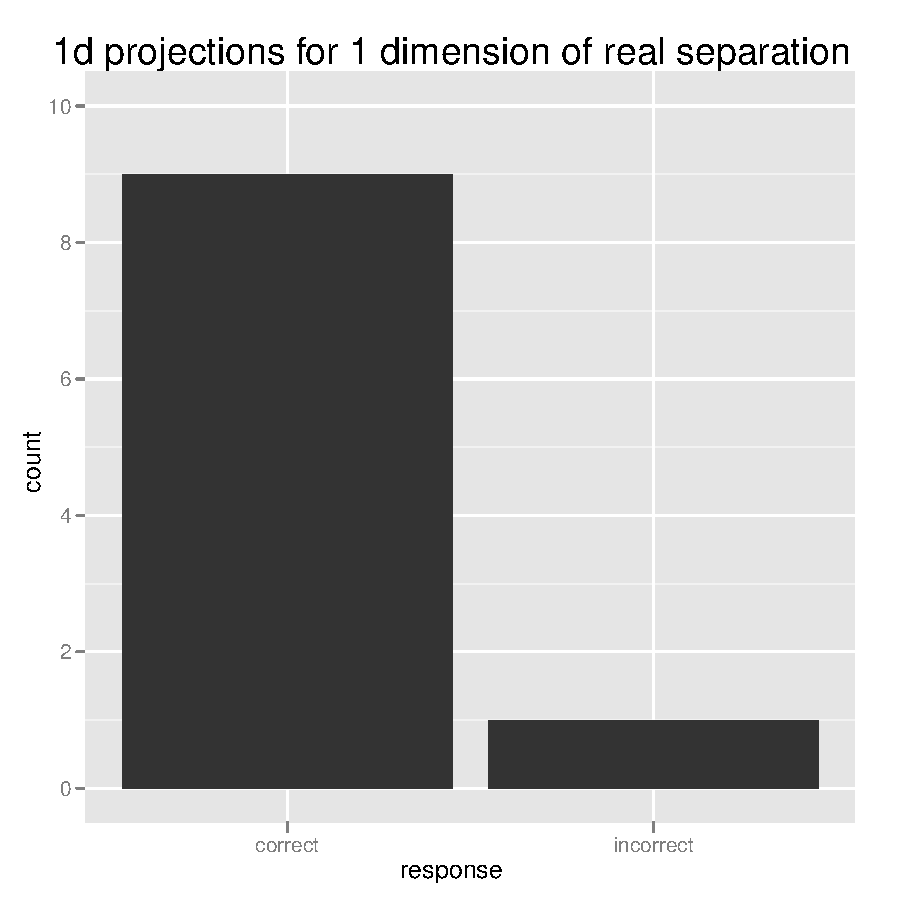
\includegraphics[width=0.25\textwidth]{result_1d_sep.pdf}}
%       \centerline{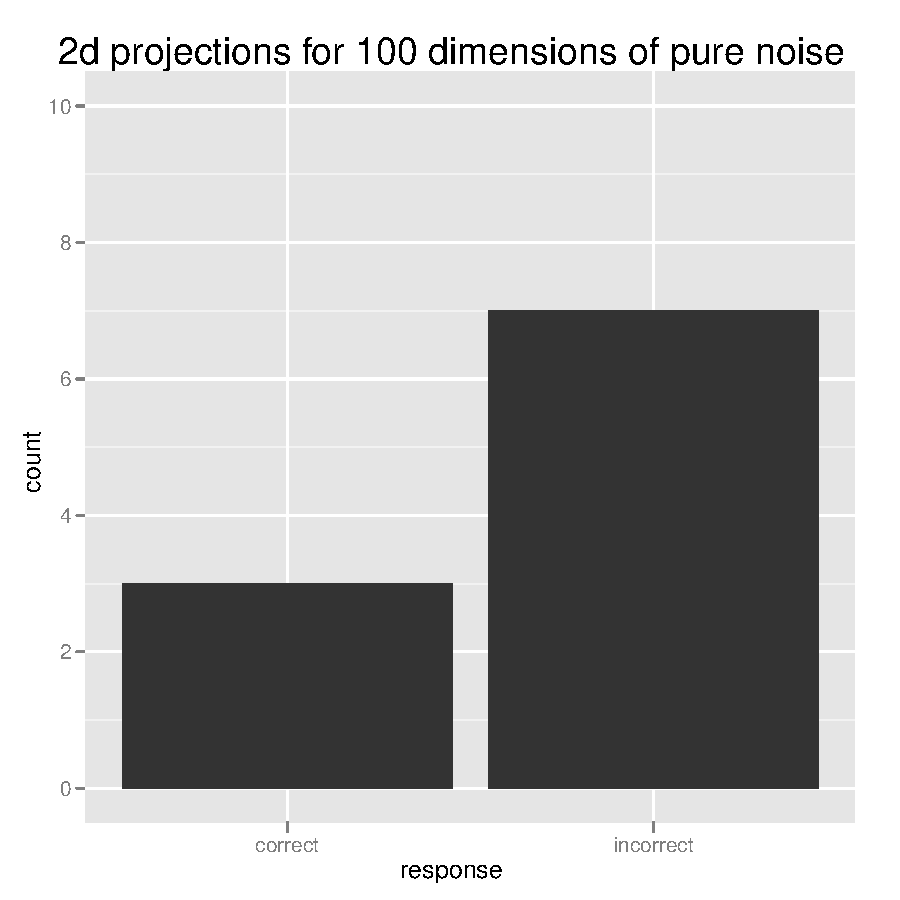
\includegraphics[width=0.25\textwidth]{result_2d_noise.pdf}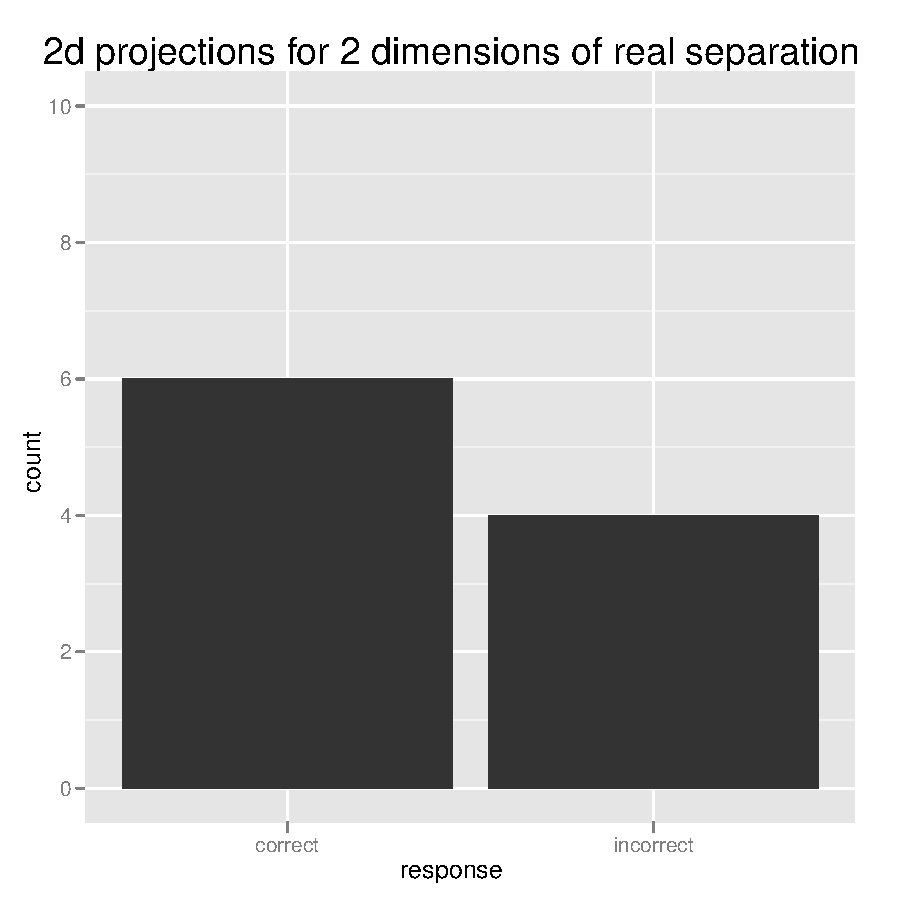
\includegraphics[width=0.25\textwidth]{result_2d_sep.pdf}}
%       \caption{Barplots showing the number of correct responses for one and two dimensional projections for data with pure noise and data with real known separation. People are more often correct in selecting the true plot when there is some real separation.  }
%       \label{fig:result}
%\end{figure}
%%\end{figurehere}



%\begin{multicols}{2}

\subsection{How do the null plots affect choices?}

We have learned that subjects tend to pick the plot in the lineup that exhibits the most separation. Figure \ref{null} examines the influence of the ($m$ - 1) null plots on this pick. Because visual inference only allows for a finite (small) number of comparisons against the sampling distribution, the inference of the null plots in the lineup is important. More details are available in \cite{roychowdhury:2012}). If a null plot has a stronger signal, subject picks that as the observed data plot. The influence of the null plots is calculated by the ratio between the minimum WBratio of the null plots and the WBratio for the observed data plot for each lineup. Figure \ref{null} shows that the proportion correct against this ratio. The vertical line acts as a reference line where the ratio is 1. The points to the right of the line should indicate easier lineups and those to the left indicate more difficult lineups. As the ease increases, the success rate increases. When there is a null plot with similar WBratio, subjects have a harder time choosing.
%Since the values of WBratio vary for each lineup depending on the presence or absence of real separation, the difference is scaled by dividing the difference by the WBratio of the observed data plot of the lineup. To put the differences on a logarithmic scale, the differences are adjusted by adding a constant term.   

%\begin{figure*}[hbtp]
%%\begin{figurehere}
%   \centering
%       \scalebox{0.6}{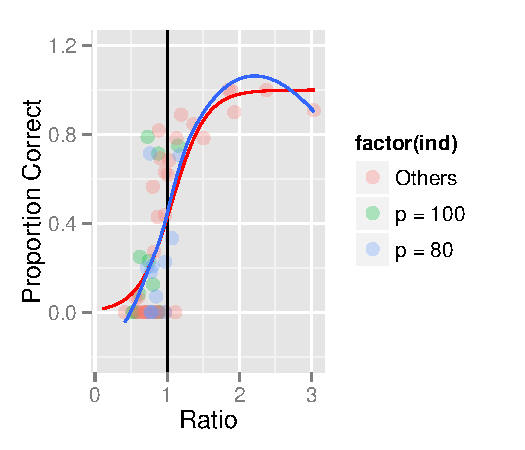
\includegraphics{suc-ratio-wbratio-glm.pdf}}
%       \caption{Proportion of correct response against the ratio of the minimum WBratio of the null plots and the WBratio of the observed data plot for each lineup. The vertical line represents ratio equal to 1 when WBratio of the observed data plot is equal to the minimum WBratio of the null plots. The points left to the line indicates a difficult lineup in the sense that at least one of the null plots had a lower WBratio value than the observed data plot. The blue line shows a logistic regression model which indicates that there is a positive effect of the ratio on the proportion correct.}
%       \label{null}
%\end{figure*}

\begin{figure}[htbp]
\centering
\mbox{\subfigure[Proportion correct vs Ratio]{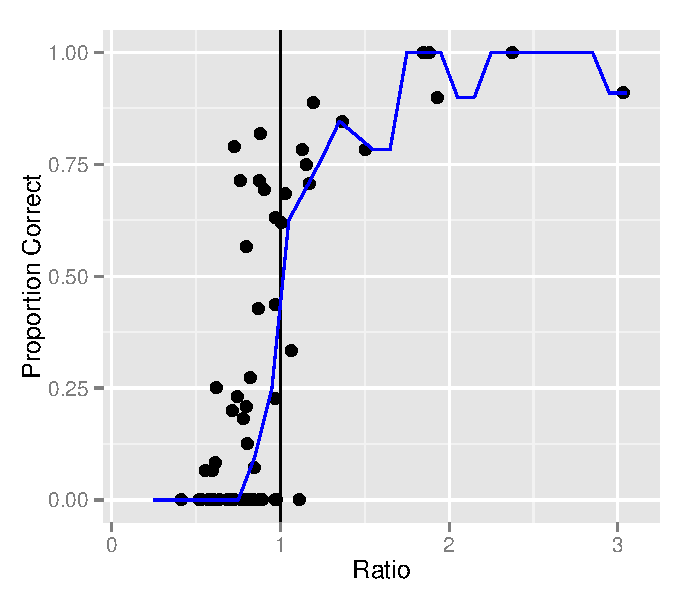
\includegraphics[width=3in]{suc-ratio-smoother.pdf}}\quad
\subfigure[Mean time vs Ratio ]{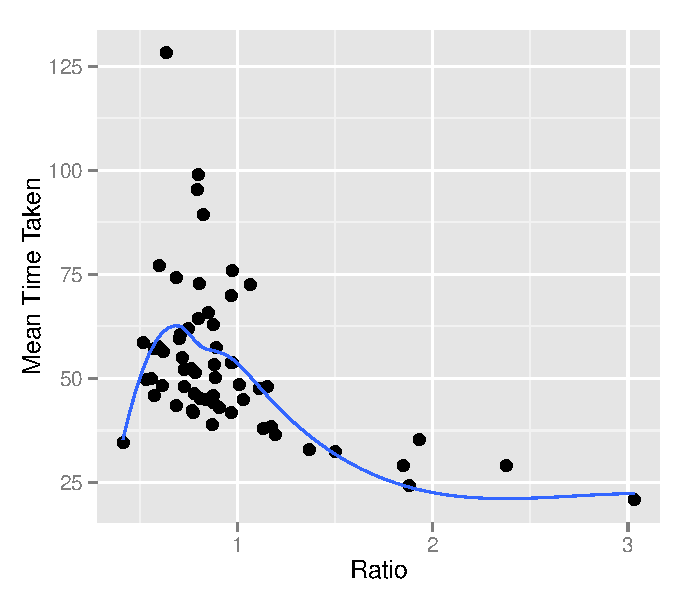
\includegraphics[width=3in]{mtime-ratio-loess.pdf} }}
\caption{(a) Proportion of correct response against the ratio of the minimum WBratio of the null plots and the WBratio of the observed data plot for each lineup. The vertical line represents ratio equal to 1 when WBratio of the observed data plot is equal to the minimum WBratio of the null plots. The points left to the line indicates a difficult lineup in the sense that at least one of the null plots had a lower WBratio value than the observed data plot. The blue line shows a median smoother which indicates that there is a positive effect of the ratio on the proportion correct. (b) Mean time taken to respond against the ratio. As the ratio increases, the mean time taken decreases indicating that the subjects have an easier time in identifying the observed data plot. } 
\label{null}
\end{figure}




\section{Wasps data, revisited. }

%\subsection{Statement of the hypothesis}

We return now to the motivating example. Figure \ref{oligo} suggested that the expression patterns of the wasp groups are different.  The question of interest is ``Is this separation real?''. This can be investigated by testing the hypothesis: 

\begin{quote}
$H_o$: There is NO difference in the expression levels between the types of wasp.\\
$H_a$: At least one of the types of wasps has different expression levels.
\end{quote}
A lineup was made of the wasp data obtained from \cite{toth:2010} to test $H_o$ where the null plots were made by permuting the wasp type label, and re-doing the LDA. If there is real difference between the expression levels for the types of wasps then the observed data plot should be detectable in the lineup. Figure \ref{toth_lineup} shows a lineup. 

\begin{figure*}[hbtp]
%\begin{figurehere}
   \centering
       \scalebox{0.90}{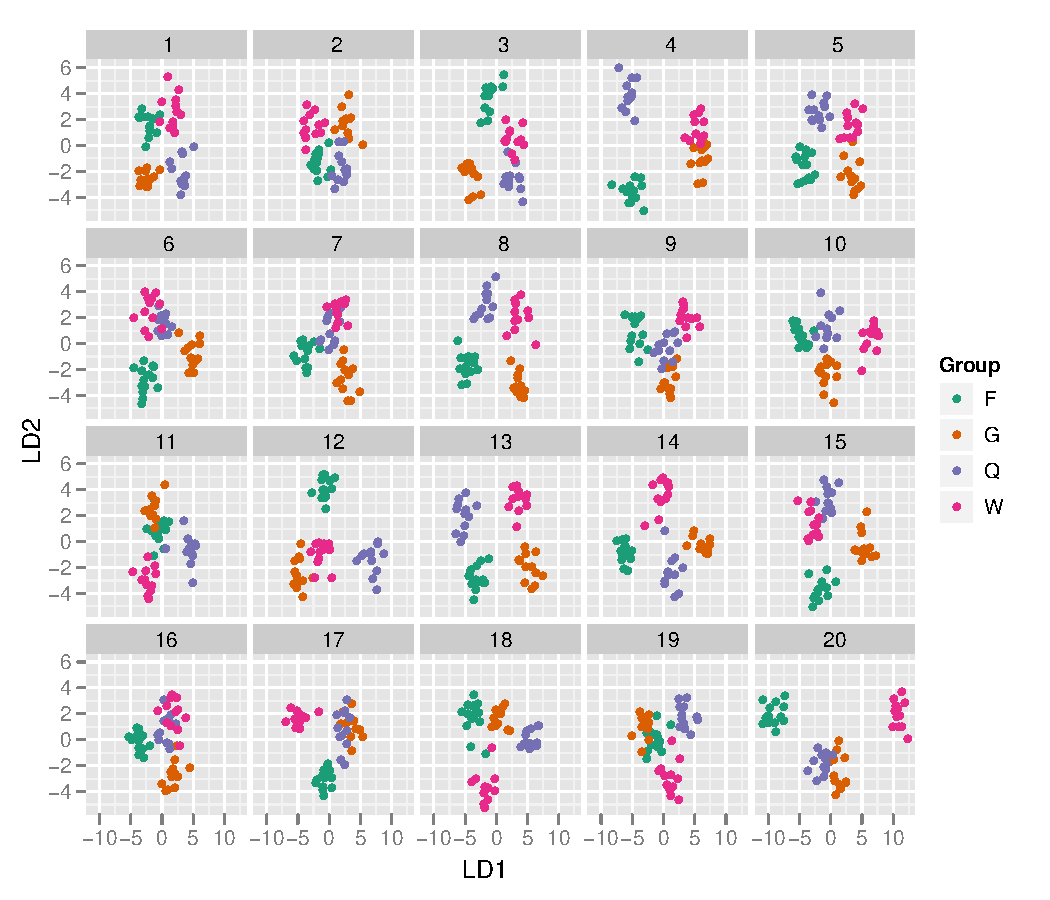
\includegraphics{toth_lineup_lda_3.pdf}}
       \caption{Lineup showing LD1 versus LD2 from an LDA on a randomly selected subset of 40 significantly different oligos. F, Foundress; G, gyne; Q, queen and W, worker. The observed data plot is placed randomly among the 19 null plots. Which plot shows the most separation between the 4 groups? The solution is provided in the Appendix.}
       \label{toth_lineup}
\end{figure*} 

This was replicated three times, to provide three different lineups, where the null plots changed but the observed data plot was the real wasps data. In addition, three more lineups were made that contained only null plots, with one plot chosen randomly to act as a observed data plot. An Amazon Turk experiment was conducted to evaluate the lineups.  A total of 116 subjects evaluated the lineups. Table \ref{wasp} shows the results. Success rate in detecting the plot of the wasp data was 0! This was worse than that of purely noise data, with the exception of one of the replicates of the purely noise data lineup. In this lineup the observed data plot (which was actually random) had more separation than any other plot in the lineup, and subjects picked up on this. The $p$-value was calculated according to the procedure given by \cite{majumder:2011}. The large $p$-values indicate that there is no statistically significant evidence to reject the null hypothesis. Thus we have to conclude that the separation in the wasp data is not real. It is purely the effect of high dimensionality. 

%So two different lineups are obtained : one where the observed data is the wasp data and the other where the observed data is ``permuted data'' obtained by permuting the wasp data. Three replicates of each are made. Each subject from the Amazon Turk was shown one of the above lineups randomly and were asked to identify the plot which has the most separation among the colored groups. They were also asked to record a reason for their choice and also a confidence level on the scale of 1 to 5.

%\subsection{Results}

%The probability of successful evaluation for the wasp data and permuted data is given in Table \ref{wasp}. As it can be seen, none of the subjects were able to identify the observed data plot in the wasp data. But around 10\% of the subjects were able to identify the observed data plot when the permuted data is used to generate the lineup.  But mainly there was one of the replicates in which subjects had a higher success rate (around 26\%). 

%\begin{figure*}[hbtp]
%%\begin{figurehere}
%   \centering
%       \scalebox{0.6}{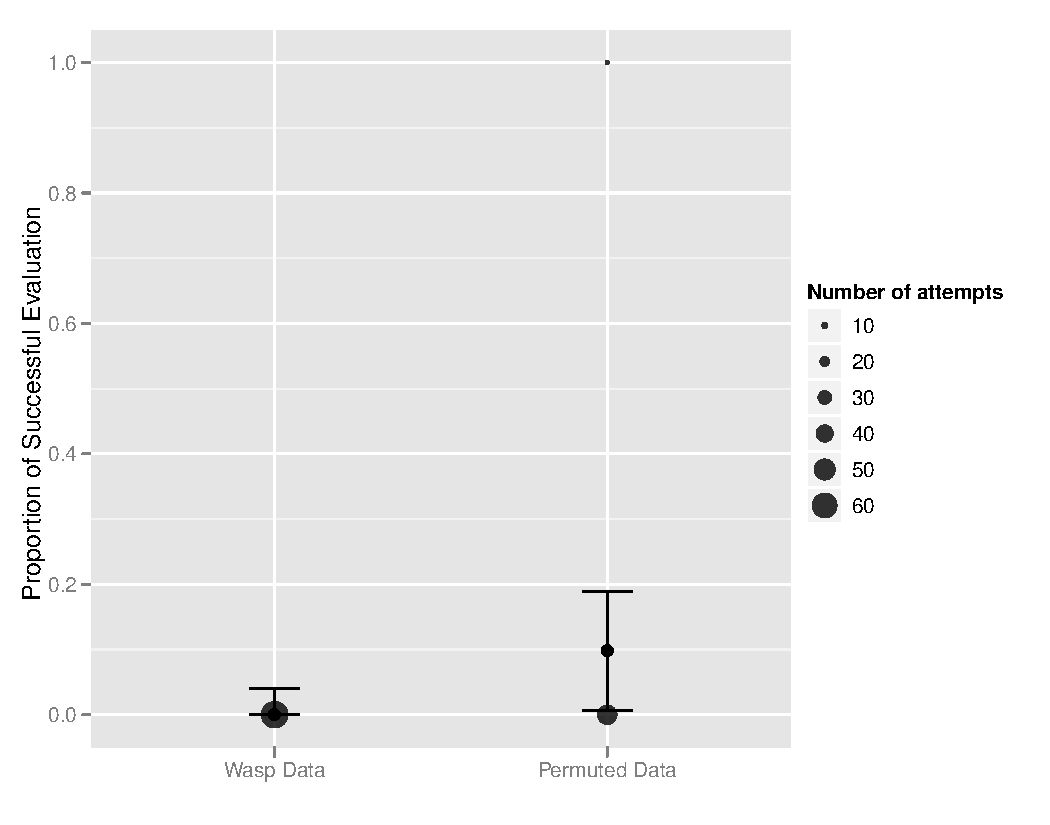
\includegraphics{wasp-result-dot.pdf}}
%       \caption{Barplot showing the probability of successful evaluation for the Wald data and the permuted data. The error bar gives the 95\% adjusted Wald intervals. }
%       \label{wasp-result}
%\end{figure*} 


%The $p$-value for a lineup is defined in \cite{majumder:2011}. Under the null hypothesis, each observer has a $1/m$ chance of picking the test statistic from the lineup, where $m$ is the number of plots in the lineup. For $K$ independent observers, let $X$ be the number of observers picking the test statistic from the lineup. Under the null hypothesis, $X$ $\sim$ $\hbox{Binom}_{K, 1/m}$, therefore the $p$-value of a lineup of size $m$ evaluated by $K$ observers is given as

%$$P(X \ge x) = 1 - \hbox{Binom}_{K, 1/m}(x - 1) = \sum_{i = x}^K {K \choose i} \left(\frac{1}{m} \right)^i \left(\frac{m - 1}{m}\right)^{K - i}$$

%Here $x$ is the number of observers selecting the observed data plot. Using the above formula, the $p$-value can be calculated for both the wasp data and the permuted data which are presented in Table \ref{wasp}.  


\begin{table}[ht]
\begin{center}
\caption{Results of the Turk study on the wasps data. Proportion of correctness of each lineup is shown, with the number of subjects, and $p$-value associated with the result. The success rate is highest for one of the purely noise lineups, which occurred because the plot with the most difference between groups happened to be the one that was randomly generated as the ``real'' data. Averaging the $p$-values for each set of lineups, for the wasps was 1.0, and for the pure noise is 0.67 suggests that the apparent separation in the wasp data is consistent with pure noise induced by the high dimensions.}
\vspace{0.15cm}
\begin{tabular}{r|r|r|rr}
\hline
  \hline
 Data & Replicate & Num Subjects & Prop Correct & $p$-value\\ 
  \hline
  & 1 & 25 & 0.0000 &  1.0000\\
Wasps & 2 & 13 & 0.0000 &  1.0000\\ 
 & 3 & 27 & 0.0000 &  1.0000\\
 \hline
 & 1 & 19 & 0.2632 &  0.0002\\
Purely noise & 2 & 18 & 0.0000 &  1.0000 \\ 
 & 3 & 14 & 0.0000 &  1.0000\\
%  noise1 & $-$3.750 & 0.298  & 0.000 \\ 
%  projection2 & $-$0.079 & 0.176  & 0.653 \\ 
   \hline
\end{tabular}
\label{wasp}
\end{center}
\end{table}

In the original paper \citep{toth:2010}, the dimensionality was reduced from much higher, by choosing the genes that showed the greatest separation. So the problem of high dimensionality is actually even worse for these data. In general, reducing the data dimensions so that the sample size is bigger than dimension is not, on its own, sufficient. It is important, even, with so few cases to do cross-validation, or break the sample into training and test sets before conducting analysis. LDA is known also to be a problem for HDLSS data, because it requires estimating more parameters than the available data allows. A better prospect for dimension reduction is the penalized discriminant analysis (PDA) index \citep{lee:2009}, which helps adjust for the over-estimation. Other results and the overall conclusions in \cite{toth:2010} are not affected by the inadequacy revealed by this visual inference analysis. A similar LDA performed on wasp gene expression data with a much higher sample size in \cite{toth:2007} did not suffer from the HDLSS problem. We determined that there were robust separations between the groups based on those data (results not shown).

%Making the number of dimensions ($p$) less than the sample size ($n$) may not solve the problem in case of LDA. Figure \ref{combin} shows that when the sample size ($n$) is 50, the probability of obtaining separated groups for purely noise data divided into 2 groups is 1 for dimension ($p$) greater than 38. When the number of dimensions ($p$) is large compared to the number of observations ($n$), the LDA method is not recommended as the separation may be just due to the high dimensions. This points out the importance of dividing the data into test and training sets.  

%In Figure \ref{toth_lineup} it can be noticed that the clusters are separated even after breaking any dependency between the groups and the variables. Since PDA is a better index than LDA in a large $p$ situation, in some situations PDA index can solve the problem of obtaining the fake separations. PDA index is used to generate another lineup using the wasp data which is presented in Figure \ref{toth_pda}. In Figure \ref{toth_pda}, the clusters are not even separated and it is difficult to identify the observed data plot. Hence when the number of dimensions $p$ is smaller or equal to the sample size $n$, it is recommended to use a PDA index instead of a LDA index. 

%\begin{figure*}[hbtp]
%%\begin{figurehere}
%   \centering
%       \scalebox{1}{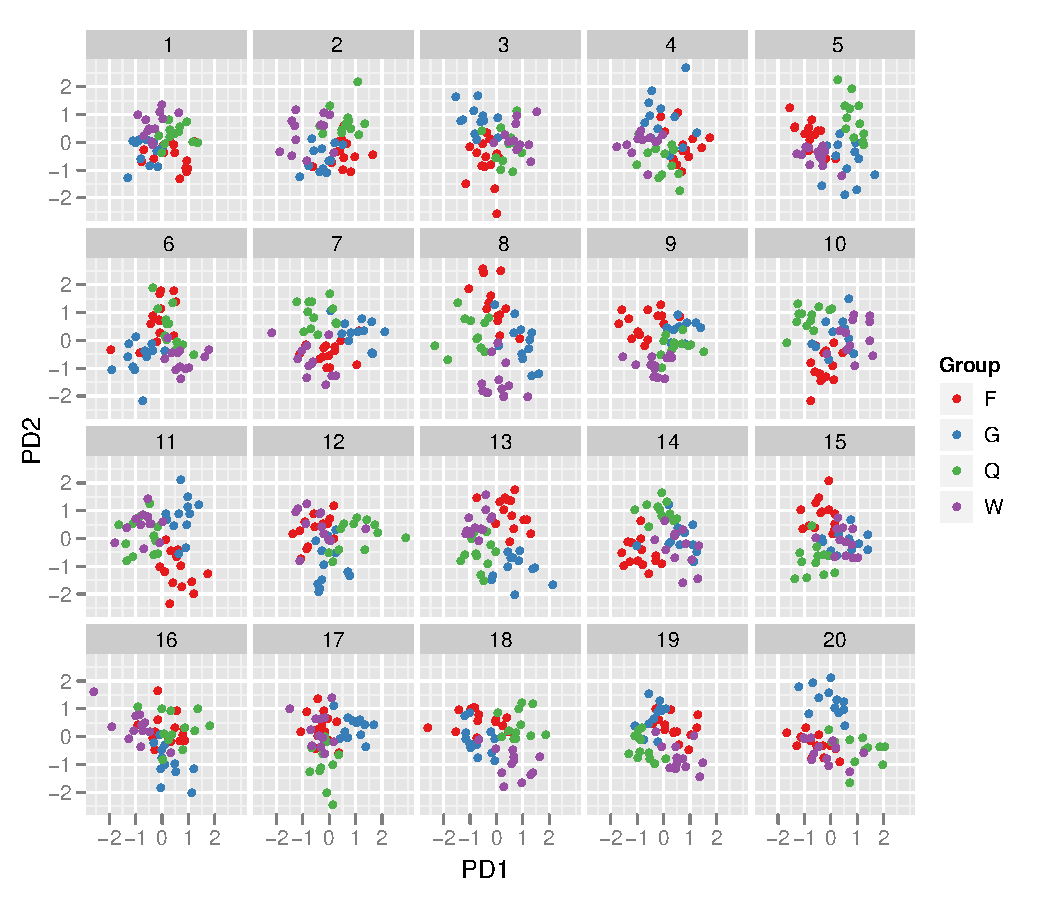
\includegraphics{toth_lineup_pda_13.pdf}}
%       \caption{Lineup showing PD1 versus PD2 from an PDA on the wasp data. Here F, Foundress; G, gyne; Q, queen and W, worker. The observed data plot is placed randomly among 19 null plots. Can you identify the plot which has the most separation between the colored groups? The solution is provided in the Appendix.  }
%       \label{toth_pda}
%\end{figure*}   



%
%\subsection{Fun Activity}
%
%{\color{red} The description of the procedure to calculate a probable bound for the number of dimension at which the groups start separating. } \\
%The previous section clearly suggests that the clusters becomes more and more visible as we increase the number of dimensions. So a natural question is ``What is the probable dimension of data when we can clearly see the two separated clusters for the one dimensional projections and the three separated clusters for the two dimensional projections." So out of our curiosity,  we consider 2 dimensions of random noise and each dimension has 30 observations with 2 classes. Hence there is 15 observations in each class. We plot the one dimensional projections and see if we can see the classes separated. We say that the two class are separated if we can draw a straight line between the two colors without touching any of them. We repeat the same procedure by increasing the number of dimensions by 1 every time. In this manner we plot the two dimensional projections for the number of dimensions from 2 to 62. Figure \ref{conf_int} shows the plots of the one dimensional projections for the number of dimensions from 23 to 42 and Figure \ref{conf_int1} shows the plots of the two dimensional projections for $p$ ranging from 23 to 42.
%
%%\end{multicols}
%
%\begin{figure*}[hbtp]
%%\begin{figurehere}
%   \centering
%       \scalebox{0.95}{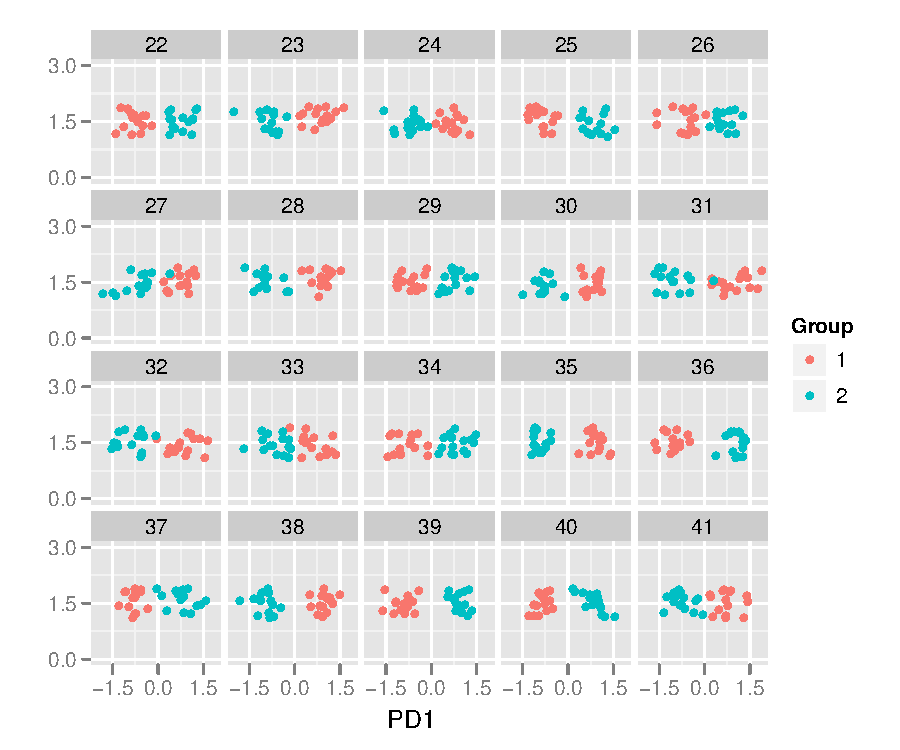
\includegraphics{plot_1d_22_41_new.pdf}}
%       \caption{Plots showing the one dimensional projections for a fixed sample size $n=30$ and the number of dimensions ranging from 23 to 42. The number written above the plot is the number of dimension. Can you see where the colors starts separating?  }
%       \label{conf_int}
%\end{figure*}
%
%\begin{figure*}[hbtp]
%%\begin{figurehere}
%   \centering
%       \scalebox{0.95}{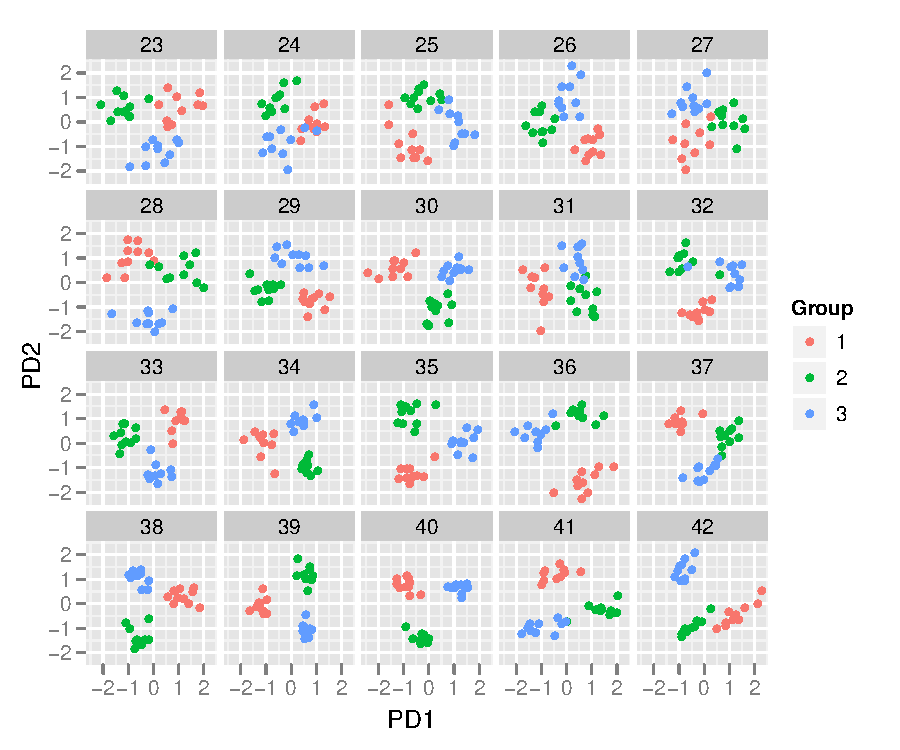
\includegraphics{plot_2d_23_42_new.pdf}}
%       \caption{Plots showing the two dimensional projections for a fixed sample size $n=30$ and the number of dimensions ranging from 23 to 42. The number written above the plot is the number of dimension. Can you see where the colors starts separating?  }
%       \label{conf_int1}
%\end{figure*}
%
%%\begin{multicols}{2}
% 
%Now we see the plot where the one dimensional projections shows a separation between the colors. We draw 100 such plots and note the number of dimension at which the classes separate out. We take the 5th and the 95th percentile of these numbers to obtain a probable range of the dimension at which the clusters are formed.
%
%Similarly we take 3 dimensions of pure noise with 30 observations in each dimension. Each dimension is divided into 3 classes, with 10 observations in each class. We plot the two dimensional projections and see whether the classes are separated. We again define the classes to be separate if we can draw three lines making an angle of $120^{\circ}$ among themselves without touching any color. So the classes will be separated if none of the colors overlap. We again repeat the same procedure by increasing the number of dimensions by 1 every time. We plot the two dimensional projections from 3 to 62 for sample size 30. We again make 100 such plots and note the number of dimension at which the classes start separating. 
%
%{\color{red} Explanation of the findings. } \\
%Hence a probable range that we obtain from the 100 plots for the one dimensional projection is between 24 and 34 and the a probable range for the two dimensional projection is between 26 and 36.

%\subsection{Probability of observing random groups using LDA} \label{sec:distance}

%\subsection{Procedure}
%topic
%{\color{red} Description of the procedure to look at the distance between the groups as we increase the number of dimension for a data with no real separation.} \\
\section{Conclusions}

The purpose of this paper has been to apply the visual inference methods for dimension reduction using projection pursuit. HDLSS data requires dimension reduction and LDA is the classical method for this. However for high dimension and small sample size, LDA provides separation even for data with no separation. Figure \ref{dist_1d} illustrates this. Figure \ref{dist_1d} shows the one dimensional projections (LD1) for four different values of dimension ($p = 2, 20, 50, 100$) for a sample size of 30. For a fixed sample size with 2 groups for data without any separation, the groups separate as the number of dimension increases. The separation is not real but this only happens due to the large dimensions. It would be interesting to calculate an interval for the dimension at which the group starts separating for a data with no separation using a visual method. Future work may explore this.

%\end{multicols}
%
%%\newpage
%%
\begin{figure*}[hbtp]
%\begin{figurehere}
   \centering
	\scalebox{0.25}{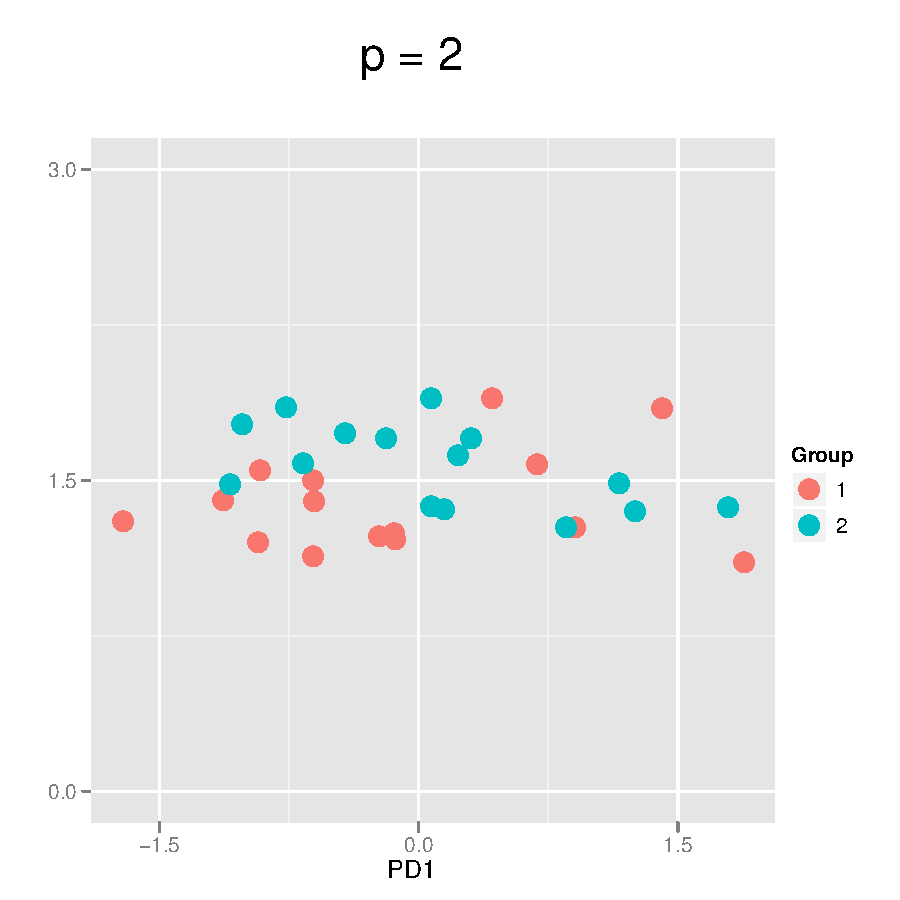
\includegraphics{plot_1d_2.pdf}}
	\scalebox{0.25}{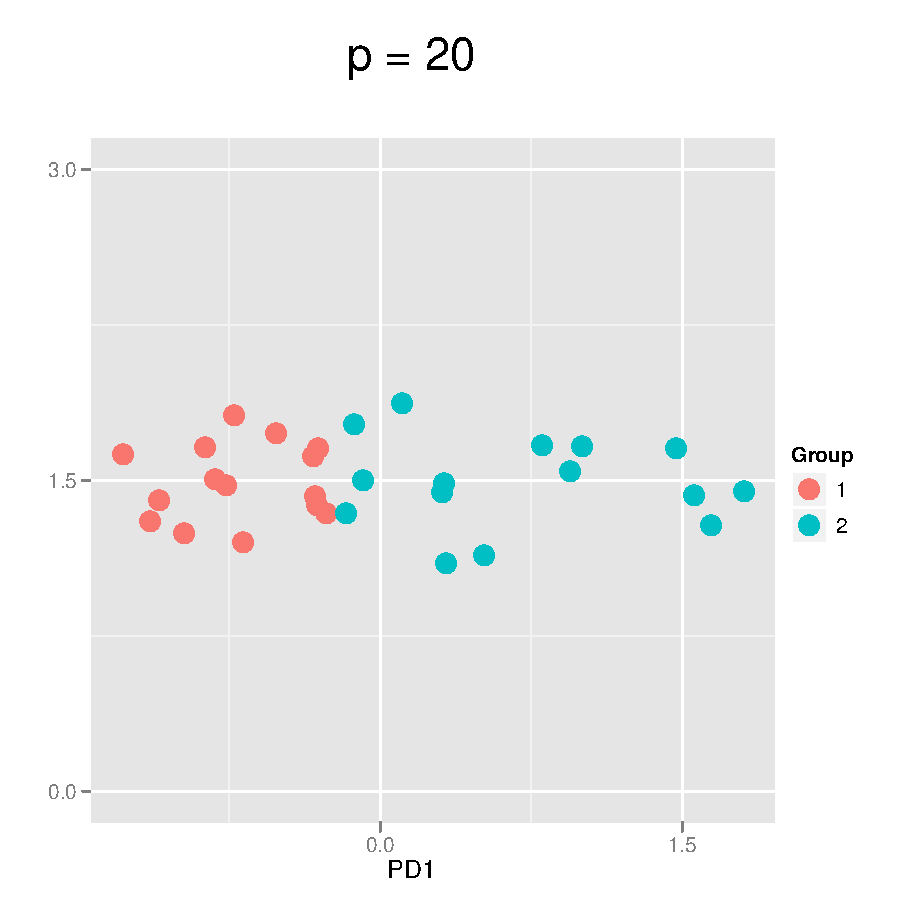
\includegraphics{plot_1d_20.pdf}}
	\scalebox{0.25}{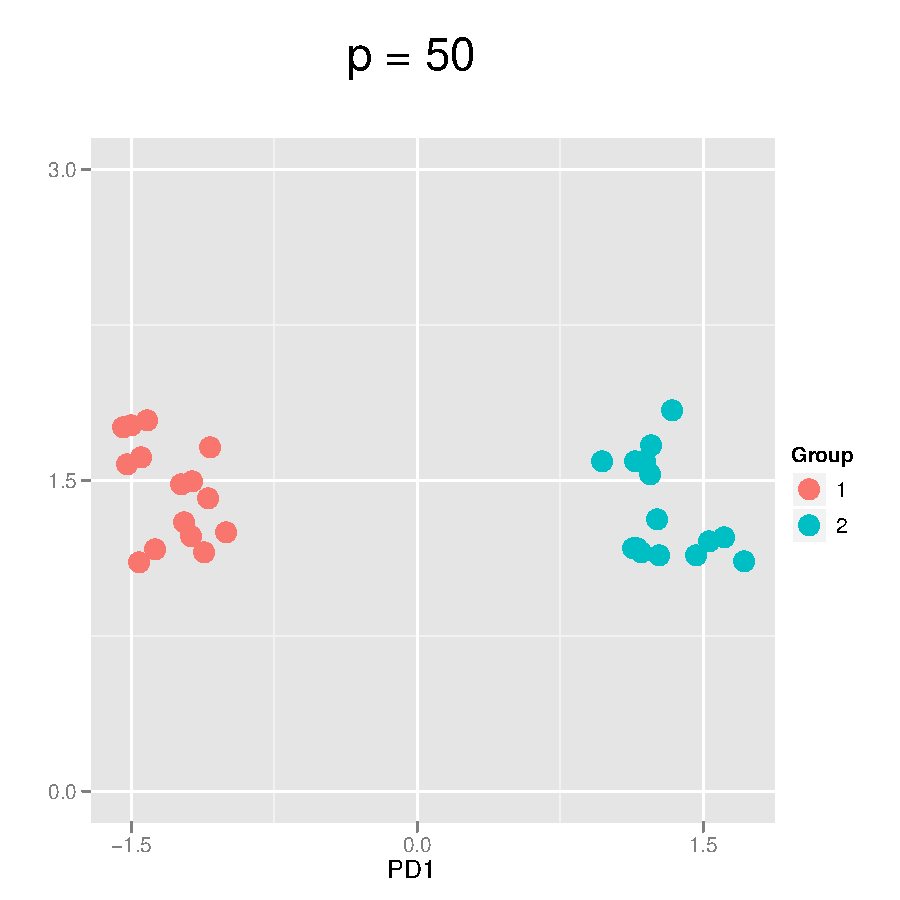
\includegraphics{plot_1d_50.pdf}}
	\scalebox{0.25}{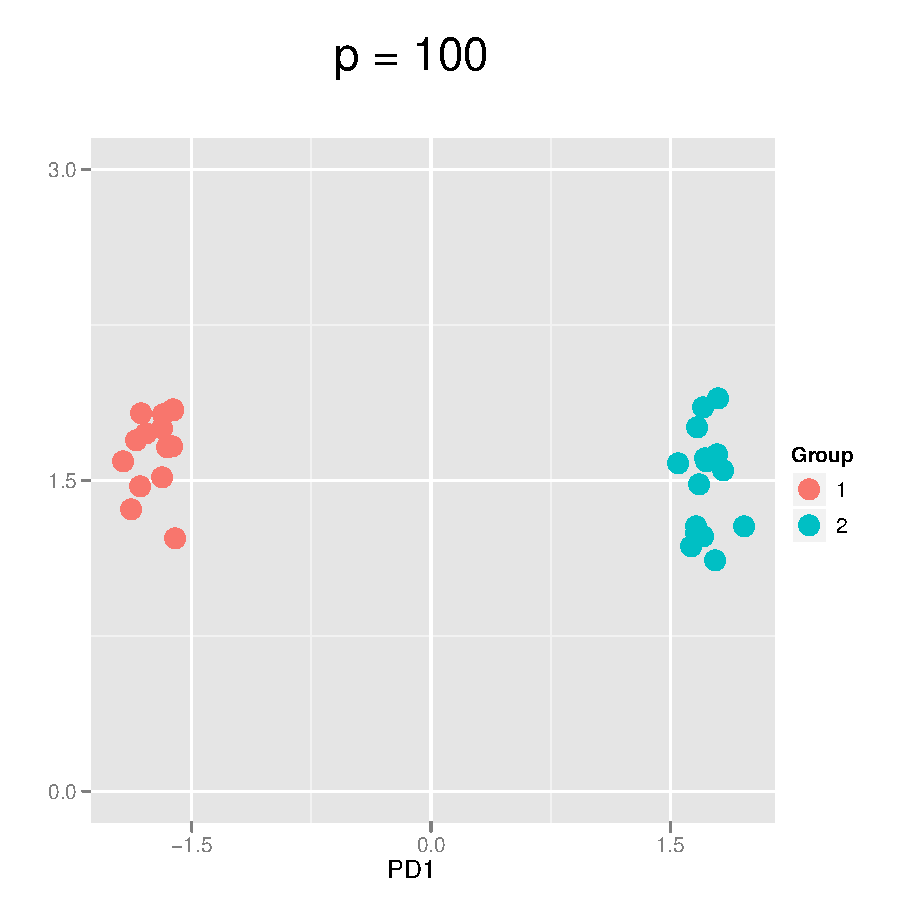
\includegraphics{plot_1d_100.pdf}}
% \scalebox{0.25}{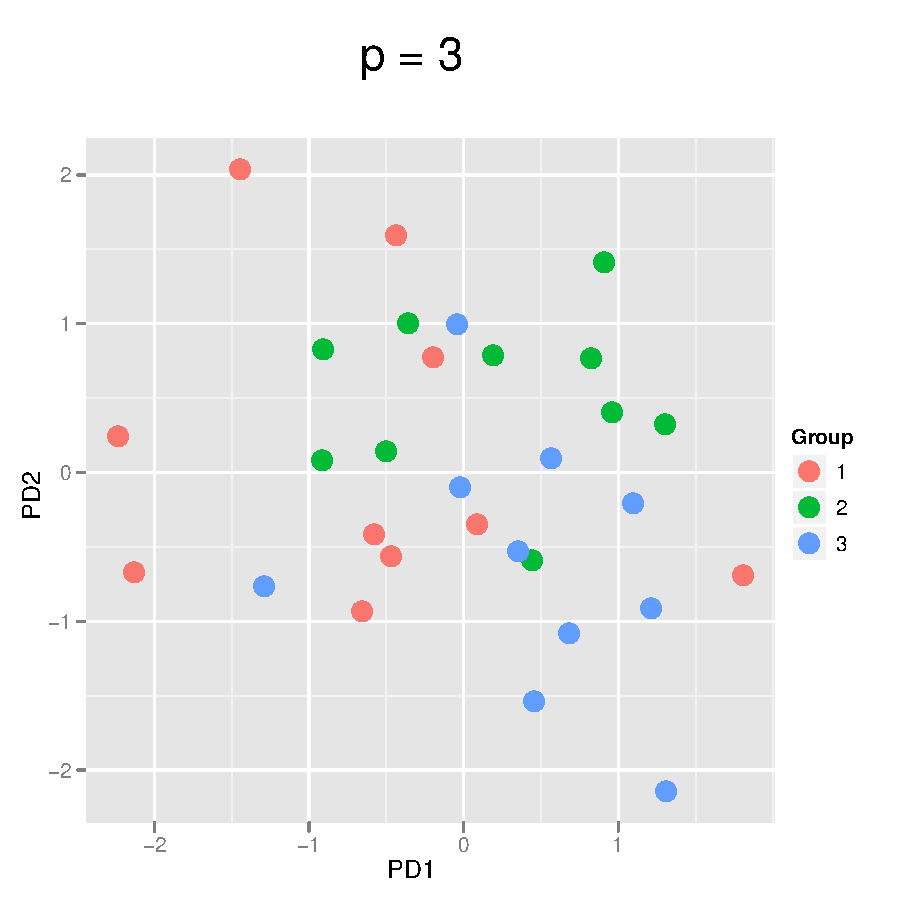
\includegraphics{plot_2d_3.pdf}}
%	\scalebox{0.25}{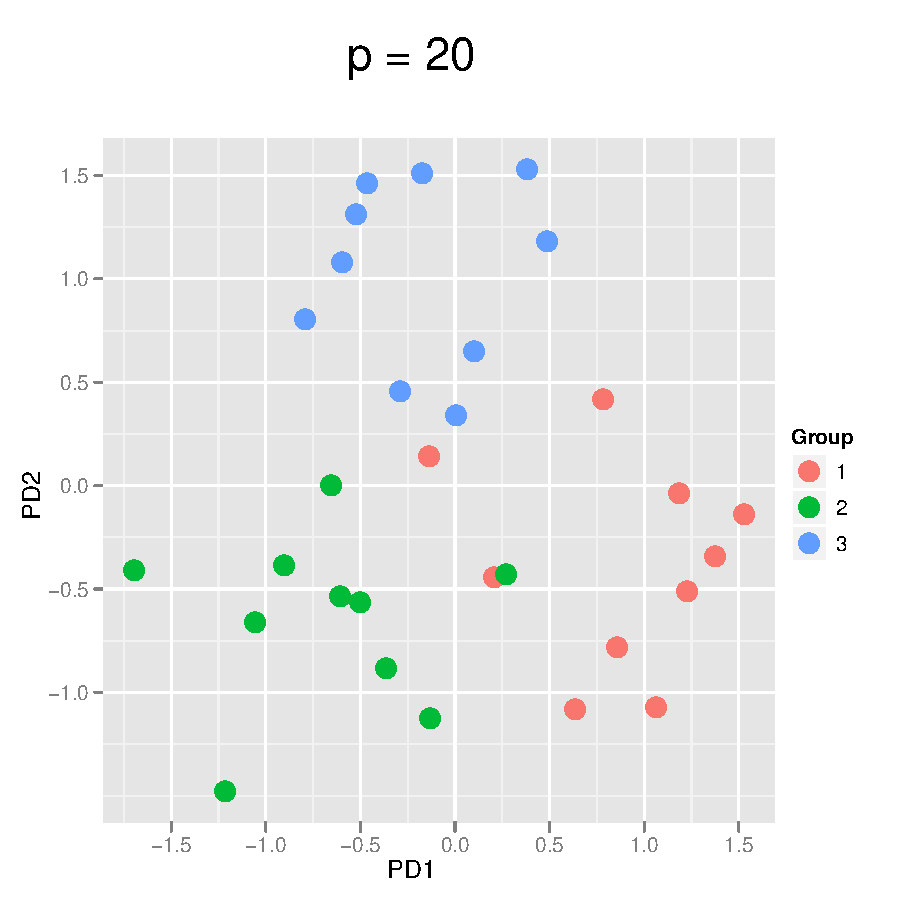
\includegraphics{plot_2d_20.pdf}}
%	\scalebox{0.25}{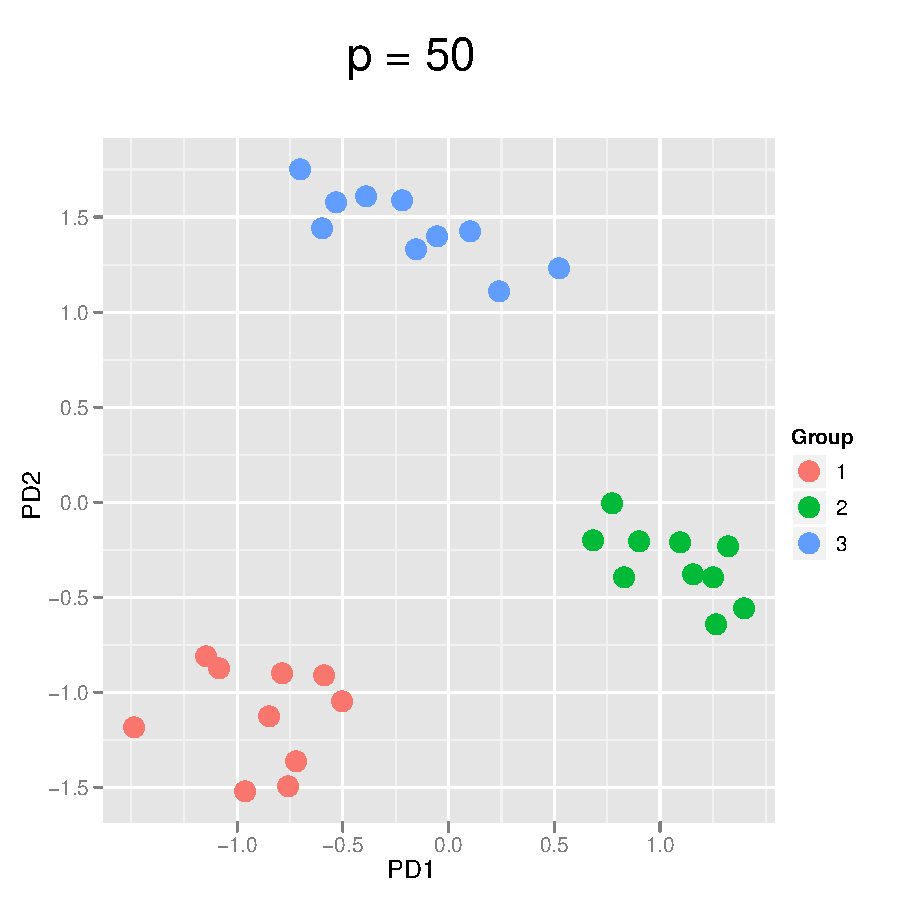
\includegraphics{plot_2d_50.pdf}}
%	\scalebox{0.25}{\includegraphics{plot_2d_100.pdf}}
       \caption{Plots showing one dimensional projections for 4 different values of dimension $p=3$, $p=20$, $p=50$ and $p=100$. The groups look more and more separated as dimension increases although the data is purely noise.  }
       \label{dist_1d}
\end{figure*}

%\begin{multicols}{2}
%{\color{red} Description for two dimensional projections.} \\
%Similarly, consider 3 dimensions of data with purely noise, each dimension having 30 observations divided into 3 groups with 10 observations in each group. The projection pursuit is performed as discussed above on the data and the two dimensional projections are plotted in a scatterplot. Similarly, in this case the 3 colors starts separating out as the number of dimensions increases.  Figure \ref{dist_1d} also shows the two dimensional projections for $p=3$, $p=20$, $p=50$ and $p=100$.

Interestingly, the optimal number of dimensions for which the LDA index will be unreliable given a fixed sample size $n$ can be calculated. \cite{ripley:1996} proposes a combinatorial method to compute the probability that $n$ observations with $p$ dimensions divided into 2 groups are linearly separable. 
%$$\hbox{Prob}(n, p) = \frac{1}{2^{n - 1}} \sum_{i = 0}^{\hbox{min}(n - 1, p)}{n - 1\choose i}$$
Using the formula provided in \cite{ripley:1996},  the probability of obtaining fake separation for 2 groups is 1 when the number of dimension($p$) is 25 for $n = 30$ and when $p = 38$ for $n = 50$. When the number of dimensions are 14 for $n = 30$ and 24 for $n = 50$ respectively, we have a 50\% chance of obtaining fake groups. In this paper visual inference makes this clearer.

%\begin{figure*}[hbtp]
%%\begin{figurehere}
%   \centering
%       \scalebox{0.45}{\includegraphics{probability-n-p.pdf}}
%       \caption{Probability that $n =30$ and $n = 50$ randomly chosen observations with $p$ dimensions randomly divided into two groups are linearly separable. For $n = 30$, when $p = 14$, the probability of obtaining linearly separable groups is 0.5 and for $n = 50$, the probability is 0.5 when $p = 24$ which are represented by the blue vertical lines. }
%       \label{combin}
%\end{figure*}

%\end{multicols}



%\begin{figure*}[hbtp]
%%\begin{figurehere}
%   \centering
%	\scalebox{0.25}{\includegraphics{plot-true3.pdf}}
%	\scalebox{0.25}{\includegraphics{plot-true20.pdf}}
%	\scalebox{0.25}{\includegraphics{plot-true50.pdf}}
%	\scalebox{0.25}{\includegraphics{plot-true100.pdf}}
%       \caption{Plots showing two dimensional projections for 4 different number of dimensions $p=3$, $p=20$, $p=50$ and $p=100$. Note that, like the one dimensional projections, the classes look more and more separated as we increase the number of dimensions when actually there is no real separation.  }
%       \label{dist_2d}
%\end{figure*}

%\begin{multicols}{2}
 


%{\color{red} Concluding remarks summarizing the different findings.} \\
A human subjects experiment was conducted and the subjects were recruited from \cite{turk}. The goal of the experiment was to determine how well real separation is distinguishable from random noise. The responses of the subjects were recorded and the results were analyzed. The proportion of correct response was higher for data with separation. For data with real separation, as the dimension increases, the proportion of correct response decreases while for data with no separation, the proportion tends to stay flat across dimensions. The projection does not have a significant effect on the responses. The subjects were equally successful in identifying the separation in 1D or 2D projections.
%Subject specific proportions of each subject was also computed. The performance of the subjects has a large variation. Though some of the subjects do very badly, but there were some subjects who performed exceedingly well. There were no restrictions  placed on the ability of the Turk workers. It was also noticed that some subjects chose the plot which has the largest separation in the groups though it may be in the null plots and not the observed data plot.
Rotation of the groups in the 2D projections were a concern. It was believed that the rotation may affect the decision of the subjects. But it was learned that the performance of the subjects was not significantly different for the 1D and 2D projections which indicates that the rotation in the lineups with 2D projection does not affect the response of the subjects. The amount of time taken to respond was higher for data without separation. But as dimension increases for data with separation, the amount of time taken is similar to the time taken for data which is purely noise. 
The subjects tend to pick plots in a lineup which has the largest separation. The difficulty of a lineup also has a significant positive effect on the proportion of successful response. The difficulty depends on the null plots obtained corresponding to the observed plot. In this paper the difficulty was calculated on the basis of the measure WBratio which was calculated for each plot in each lineup. For more details on this, see \cite{roychowdhury:2012}.

The visual inference method was also used to test whether the separation obtained among the groups is real or fake. Here the example of the paper wasp was used. It was noticed that only by making the number of dimensions less than the sample size may not always solve the problem of obtaining fake separation. Visual inference may help in communicating these large $p$, small $n$ issues. 

%The visual method may also be applied to other large $p$, small $n$ situations like bioinformatics and genetics.

\section{Appendix}

\subsection{Solution}
\begin{itemize}
\item The solution to the lineup at Figure \ref{lineup} is Plot 16. 
\item The solution to the lineup at Figure \ref{fig:test_category_1d} is Plot 11.
\item The solution to the lineup at Figure \ref{fig:test_category} is Plot 15.
\item The solution to the lineup at Figure \ref{toth_lineup} is Plot 3.
%\item The solution to the lineup at Figure \ref{toth_pda} is Plot 13.


\end{itemize}

\subsection{Choice of dimensions} \label{sec:theory}

To decide on the levels of dimension to use, the distribution of the absolute difference of the means of the two groups of a purely noise data is looked at. In this case one dimension of purely noise is considered which is divided into two groups. The means of the observations in each group is calculated. Since we are interested in the projections, the absolute differences of the means is considered.

Let us denote $X_{ij}$ as the $j$-th observation in the $i$-th group where $j = 1, \dots, n_i$. Essentially in our case there are only $i = 2$ groups. $X_{ij}$s are purely noise obtained from a standard normal distribution. The difference between the means of the purely noise data for the two groups, group 1 and group 2 is given by $\bar{X}_{1.} - \bar{X}_{2.}$ and $$\bar{X}_{1.} - \bar{X}_{2.} \sim \hbox{Normal}(0, 1/n_1 + 1/n_2)$$ where $n_1 = n_2 = 15$. So we have $$\bar{X}_{1.} - \bar{X}_{2.} \sim \hbox{Normal}(0, 2/15)$$ Let us define $$Y  = |\bar{X}_{1.} - \bar{X}_{2.}|$$ where $Y \sim \hbox{Half Normal}$ with scale parameter $ \sigma = \sqrt{1/n_1 + 1/n_2} = \sqrt{2/15}$. \\

The expectation and the variance of $Y$ can be calculated: 
$$E(Y) = \sigma \sqrt{2/\pi}$$
$$Var(Y) = \sigma^2 (1 - 2/\pi)$$

Let us consider $p$ dimensions of purely noise data, each dimension being divided into $i = 2$ groups with $n_i = 15$ observations. Let us define $$Y_m = |\bar{X}_{m1.} - \bar{X}_{m2.}|$$ where $X_{mij}$ is the $j$-th observation in the $i$-group for the $m$-th dimension. The sum of the absolute difference between the means is obtained for all the $p$ dimensions. So, define $$Y = \sum_{m=1}^p Y_m = \sum_{m=1}^p |\bar{X}_{m1.} - \bar{X}_{m2.}| $$ \\

Assuming independence among the dimensions of purely noise data,

$$E(Y) = p \sigma \sqrt{2/\pi}$$
$$Var(Y) = p \sigma^2 (1 - 2/\pi)$$

To check for the optimization procedure one dimension of real separation is considered in the data. To bring in the real separation, we adjust the mean of $X_{ij}$. We subtract any value $c$ from the mean of the first 15 observations (group 1) and add $c$ to the mean of the last 15 observations (group 2). So we define
$$X_{ij}^* \sim \hbox{Normal}(- c, 1) \qquad \hbox{for} \qquad j = 1, \dots, n_1$$
$$X_{ij}^* \sim \hbox{Normal}(c, 1) \qquad \hbox{for} \qquad j = 1, \dots, n_2$$ 
Hence we have $$\bar{X}_{1.}^* - \bar{X}_{2.}^* \sim \hbox{Normal}(2c, 1/n_1 + 1/n_2)$$ where $n_1 = n_2 = 15$. Let us define $$Y^*  = |\bar{X}_{1.}^* - \bar{X}_{2.}^*|$$ where $Y^* \sim \hbox{Folded Normal Distribution}$ with scale parameter $ \sigma = \sqrt{1/n_1 + 1/n_2} = \sqrt{2/15}$.  \\

The expectation and the variance of $Y^*$ can be calculated :

$$E(Y^*) = \sigma \sqrt{2/\pi} \exp(- 2c^2/\sigma^2) + 2c[1 - \Phi(-2c/\sigma)]$$
$$Var(Y^*) = 4c^2 + \sigma^2 - (E(Y^*))^2$$


Now the means of $X_{mij}$s are adjusted in the $p$-th dimension. So we define $Z$ as the sum of the absolute differences of the mean with one dimension of real separation as $$Z = \sum_{m=1}^{p-1} |\bar{X}_{m1.} - \bar{X}_{m2.}| + Y_p$$ where $Y_p$ follows a Folded Normal Distribution.

Again assuming independence among the dimensions of purely noise data and data with real separation,

$$E(Z) = (p - 1) \sigma \sqrt{2/\pi} + \sigma \sqrt{2/\pi} \exp(- 2c^2/\sigma^2) + 2c[1 - \Phi(-2c/\sigma)]$$
$$Var(Z) = (p - 1)\sigma^2 (1 - 2/\pi) + 4c^2 + \sigma^2 - \left( \sigma \sqrt{2/\pi} \exp(- 2c^2/\sigma^2) + 2c[1 - \Phi(-2c/\sigma)]\right)^2$$

In our case, $c = 3$ and $\sigma^2 = 2/15$. Therefore,
$$\exp(- 2c^2/\sigma^2) \approx 0 \qquad \hbox{and} \qquad \Phi(-2c/\sigma) \approx 0$$
Hence,
$$E(Z) = (p - 1) \sigma \sqrt{2/\pi} + 6$$
$$Var(Z) = (p - 1)\sigma^2 (1 - 2/\pi) + \sigma^2$$
As the value of $p$ increases for a fixed $n$, the spread of $Y$ increases with a factor of the dimension $p$ and the spread of $Z$ increases as well. The means of both $Y$ and $Z$ also increase with a factor of $p$ but the expected value of the difference between $Y$ and $Z$ stays constant and is independent of the number of dimensions ($p$). 
%\begin{equation}
$$E (Z - Y) = (p - 1) \sigma \sqrt{2/\pi} + 6 - p \sigma \sqrt{2/\pi} = 6 - \sigma \sqrt{2/\pi}$$
%\end{equation}


 Figure \ref{fig:dimen} shows the phenomenon described above. In Figure \ref{fig:dimen} notice that as the number of dimensions ($p$) increases from 20 to 100, the dark blue region of the distribution of $Y$ which is greater than the 5th percentile of $Z$ increases as the variability in $Y$ and $Z$ increases as a factor of the dimension ($p$).

% As a result, the probability of obtaining two clusters for data with pure noise indicating that for a large dimension, the sum of the absolute differences of the means for random noise would be close to the sum of the absolute differences for the means with only one dimension of real separation. 

The next step is to find the number of dimension for a specific value of the common region between the two distributions. To allow some error, the value of the number of dimension $p$ is considered for which $$\hbox{P}[Y > Z_{\alpha}] = \delta$$ where $Z_{\alpha}$ is the $\alpha$-th percentile of $Z$.  So for a given value of $\delta$,  the value of $p$ is calculated for which the above condition holds true for $\alpha = 0.05$.

The above described procedure is done for 5 different values of $\delta  = 0.0000001, 0.01, 0.05, 0.1$ and $0.2$ and for each value of $\delta$, it is repeated 100 times. Table \ref{tab:dimen} shows the summaries of the number of dimensions for each value of $\delta$.

\begin{table}[htbp]
\begin{center}
\caption{Numerical summaries of dimension $p$ for each value of $\delta$. Notice that with the increase in the dark blue region $\delta$, the median number of dimensions required to obtain the region also increases. This also means for a large value of $p$ the difference between the groups for data with purely noise is close to the difference between the groups for data with real separation. }
\begin{tabular}{rrrr}
  \hline
  \hline
  $\delta$ & Median & 5th percentile & 95th percentile \\
  \hline
  0.0000001 & 24 & 19 & 28 \\
      0.01 & 41 & 38 & 44\\
   0.02 & 61 & 56 & 64 \\
     0.1 & 77 & 72 & 81\\   
     0.2 & 106 & 99 & 112\\ 
      \hline
\end{tabular}
\label{tab:dimen}
\end{center}
\end{table}



\section{Acknowledgement:}
%
This work was funded by National Science Foundation grant DMS 1007697.

%\bibliographystyle{plainnat}
\bibliographystyle{spbasic}
%%\bibliographystyle{ieeetr}
\bibliography{references}

\end{document}
